\setchapterimage[6.5cm]{icecube}
\setchapterpreamble[u]{\margintoc}
\chapter{Neutrinos in IceCube and DeepCore}
\labch{icecube}
% \begin{fquote}[Roald Amundsen][The South Pole][1912] We must always remember with gratitude and admiration the first sailors who steered their vessels through storms and mists, and increased our knowledge of the lands of ice in the South.
% \end{fquote}

The IceCube Neutrino Observatory is a gigaton-scale Cherenkov detector located at the geographic South Pole in close proximity to the Amundsen-Scott South Pole Station.
Constructed over the course of several deployment seasons between 2006 and 2011, it instruments approximately one cubic-kilometer of Antarctic glacier with optical sensors that can detect faint flashes of light that are produced when charged particles travel through the ice, such as those produced by neutrino interactions.
The detector serves as both a telescope to study the astrophysical origin of neutrinos and an instrument to measure their fundamental properties.

This chapter describes the instrumentation and layout of the IceCube detector, the interactions that particles undergo when they interact with the ice, and finally the signals that these interactions produce in the detector.

\section{The IceCube in-ice Array and DeepCore}

The IceCube Neutrino Observatory consists of the so-called \emph{in-ice} array, optimized for astrophysical neutrino observations, the \emph{DeepCore} array, used primarily for the observation of atmospheric neutrinos, and the \emph{IceTop} surface array that can be used to study air showers from cosmic rays.

\subsection{The Antarctic Ice}

The detection medium of the IceCube detector is the Antarctic glacier that has formed from layers of snow being deposited top of each other over the course the past $\sim\num{100000}$ years\todo{reference}.
The weight of the upper layers compresses the lower layers into a dense, crystalline structure.
As a result, the optical properties of the ice change mostly in the direction perpendicular to the layers, forming a geological record of the atmospheric conditions of the Earth.
The transmission of light through the ice is primarily characterized by the scattering and absorption length. Within the volume of IceCube, scattering lengths vary between \SI{20}{\meter} and \SI{100}{\meter}, while absorption lengths range from \SI{100}{\meter} to \SI{400}{\meter}. Both quantities are highly correlated, such that the absorption length is approximately four times as large as the scattering length.\todo{cite ice model?}
This stratigraphy was traced at millimeter resolution using a laser dust logger deployed down seven IceCube drill holes as described by \cite{dustlogger}.
The most notable feature of the stratigraphy is the \emph{dust layer} at depths between 2000~m and 2100~m as shown in \reffig{icecube-schematic}.
The optical properties of the ice within the dust layer are particularly poor.
The ice below the dust layer where the DeepCore fiducial volume is located has the best optical properties of the entire IceCube volume.

\subsection{In-Ice Array}
The 5160 Digital Optical Modules (DOMs) that make up the IceCube in-ice array are distributed over 86 strings.
Of these, 78 are arranged on a hexagonal grid spanning an area of approximately one square-kilometer with a horizontal spacing of $\sim$150~m with respect to their closest neighboring strings\sidecite{icecube_detector_17}. Each of these strings holds 60 DOMs at depths between 1450~m and 2450~m with a 17~m vertical spacing.
The volume and instrumentation density of this array is optimized for astrophysical neutrinos that are found at energies above 1~TeV\cite{icecube_detector_17}.
The electric signals measured in each DOM are digitized  and sent to the \emph{IceCube lab (ICL)}, where the signal is processed, compressed, and sent North via satellite for offline processing.
\reffig{ic_detector} gives an overview of the detector including the IceCube Lab, the ice surface and the bedrock, and a schematic of the layout of the strings is shown in \reffig{icecube-schematic}.

\begin{figure}
	\centering 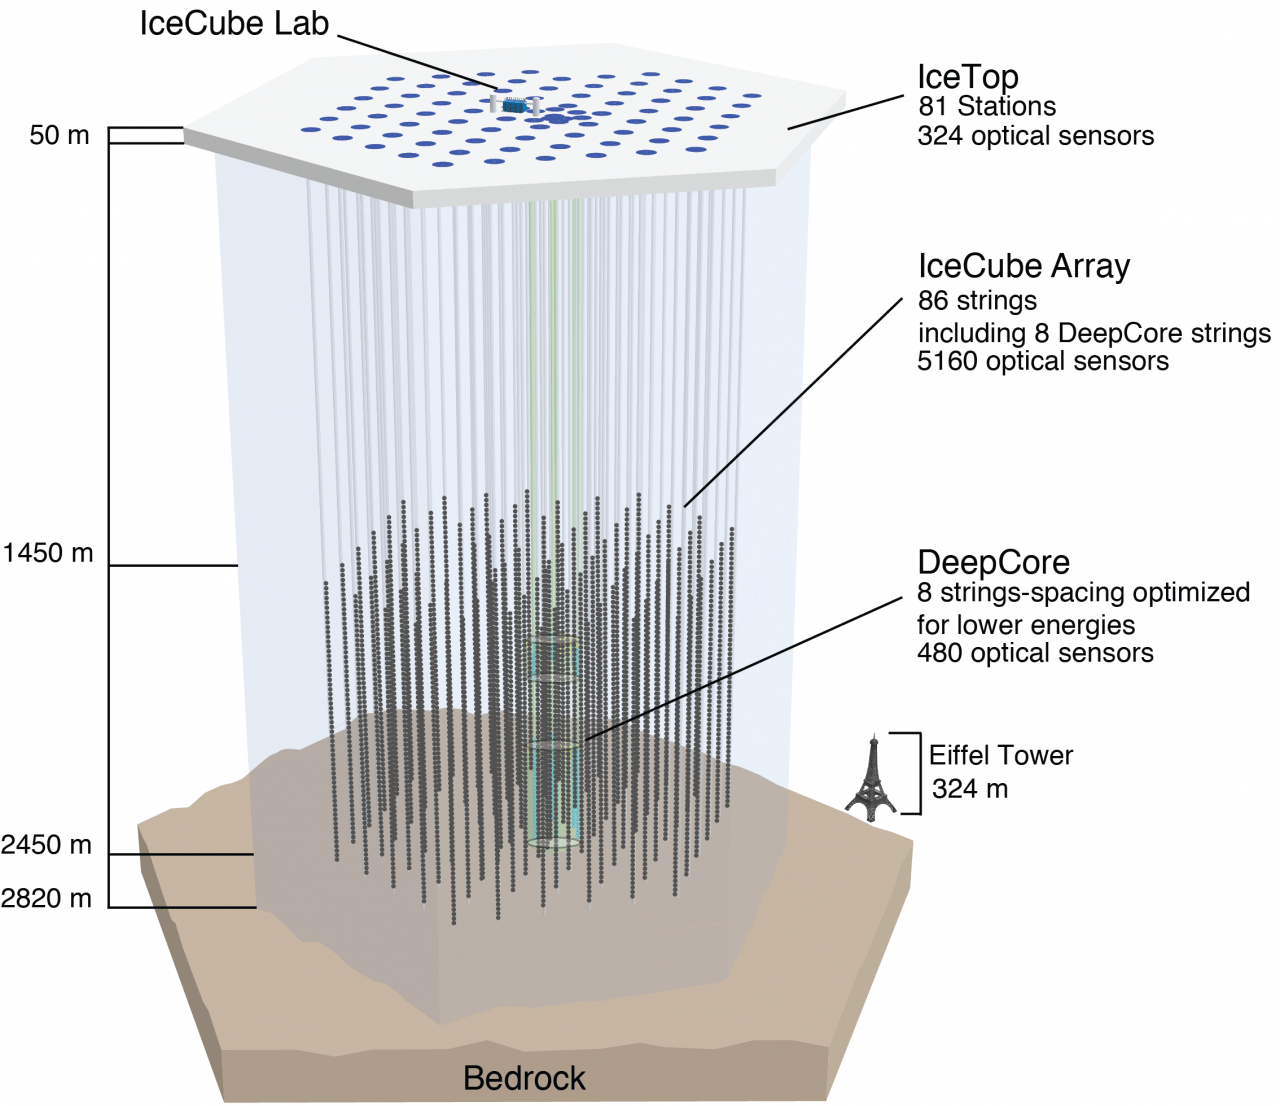
\includegraphics{figures/icecube/IceCubeArray_slim.png}
	\caption{An overview of the IceCube detector}
	\label{fig:ic_detector}
\end{figure}

\subsubsection{DeepCore}
The remaining 8 strings that are not part of the hexagonal grid are located near the center of the IceCube detector and form the \emph{DeepCore} sub-array\sidecite{DeepCore}.
The DOMs on the DeepCore strings have a higher quantum efficiency than those in the rest of the detector and are placed more closely together to lower the minimum energy threshold for neutrino observations to a few GeV.
Of the 60 DOMs on each DeepCore string, 50 are placed at depths between 2100~m and 2500~m, where the ice is the most transparent compared to the rest of the IceCube's volume (see also the side band in the bottom panel of Figure~\ref{fig:icecube-schematic}).
Together with 7 strings from the in-ice array, the DeepCore strings instrument the DeepCore 20~MT \emph{fiducial volume} as shown in the upper panel of Figure~\ref{fig:icecube-schematic}.
The remaining 10 DOMs are located at depths between 1750~m and 1850~m and are used as a veto cap to reject atmospheric muons entering the detector directly from above.
In addition, the larger hexagonal IceCube array also serves as a veto for observations inside the DeepCore fiducial volume.
\begin{figure}
    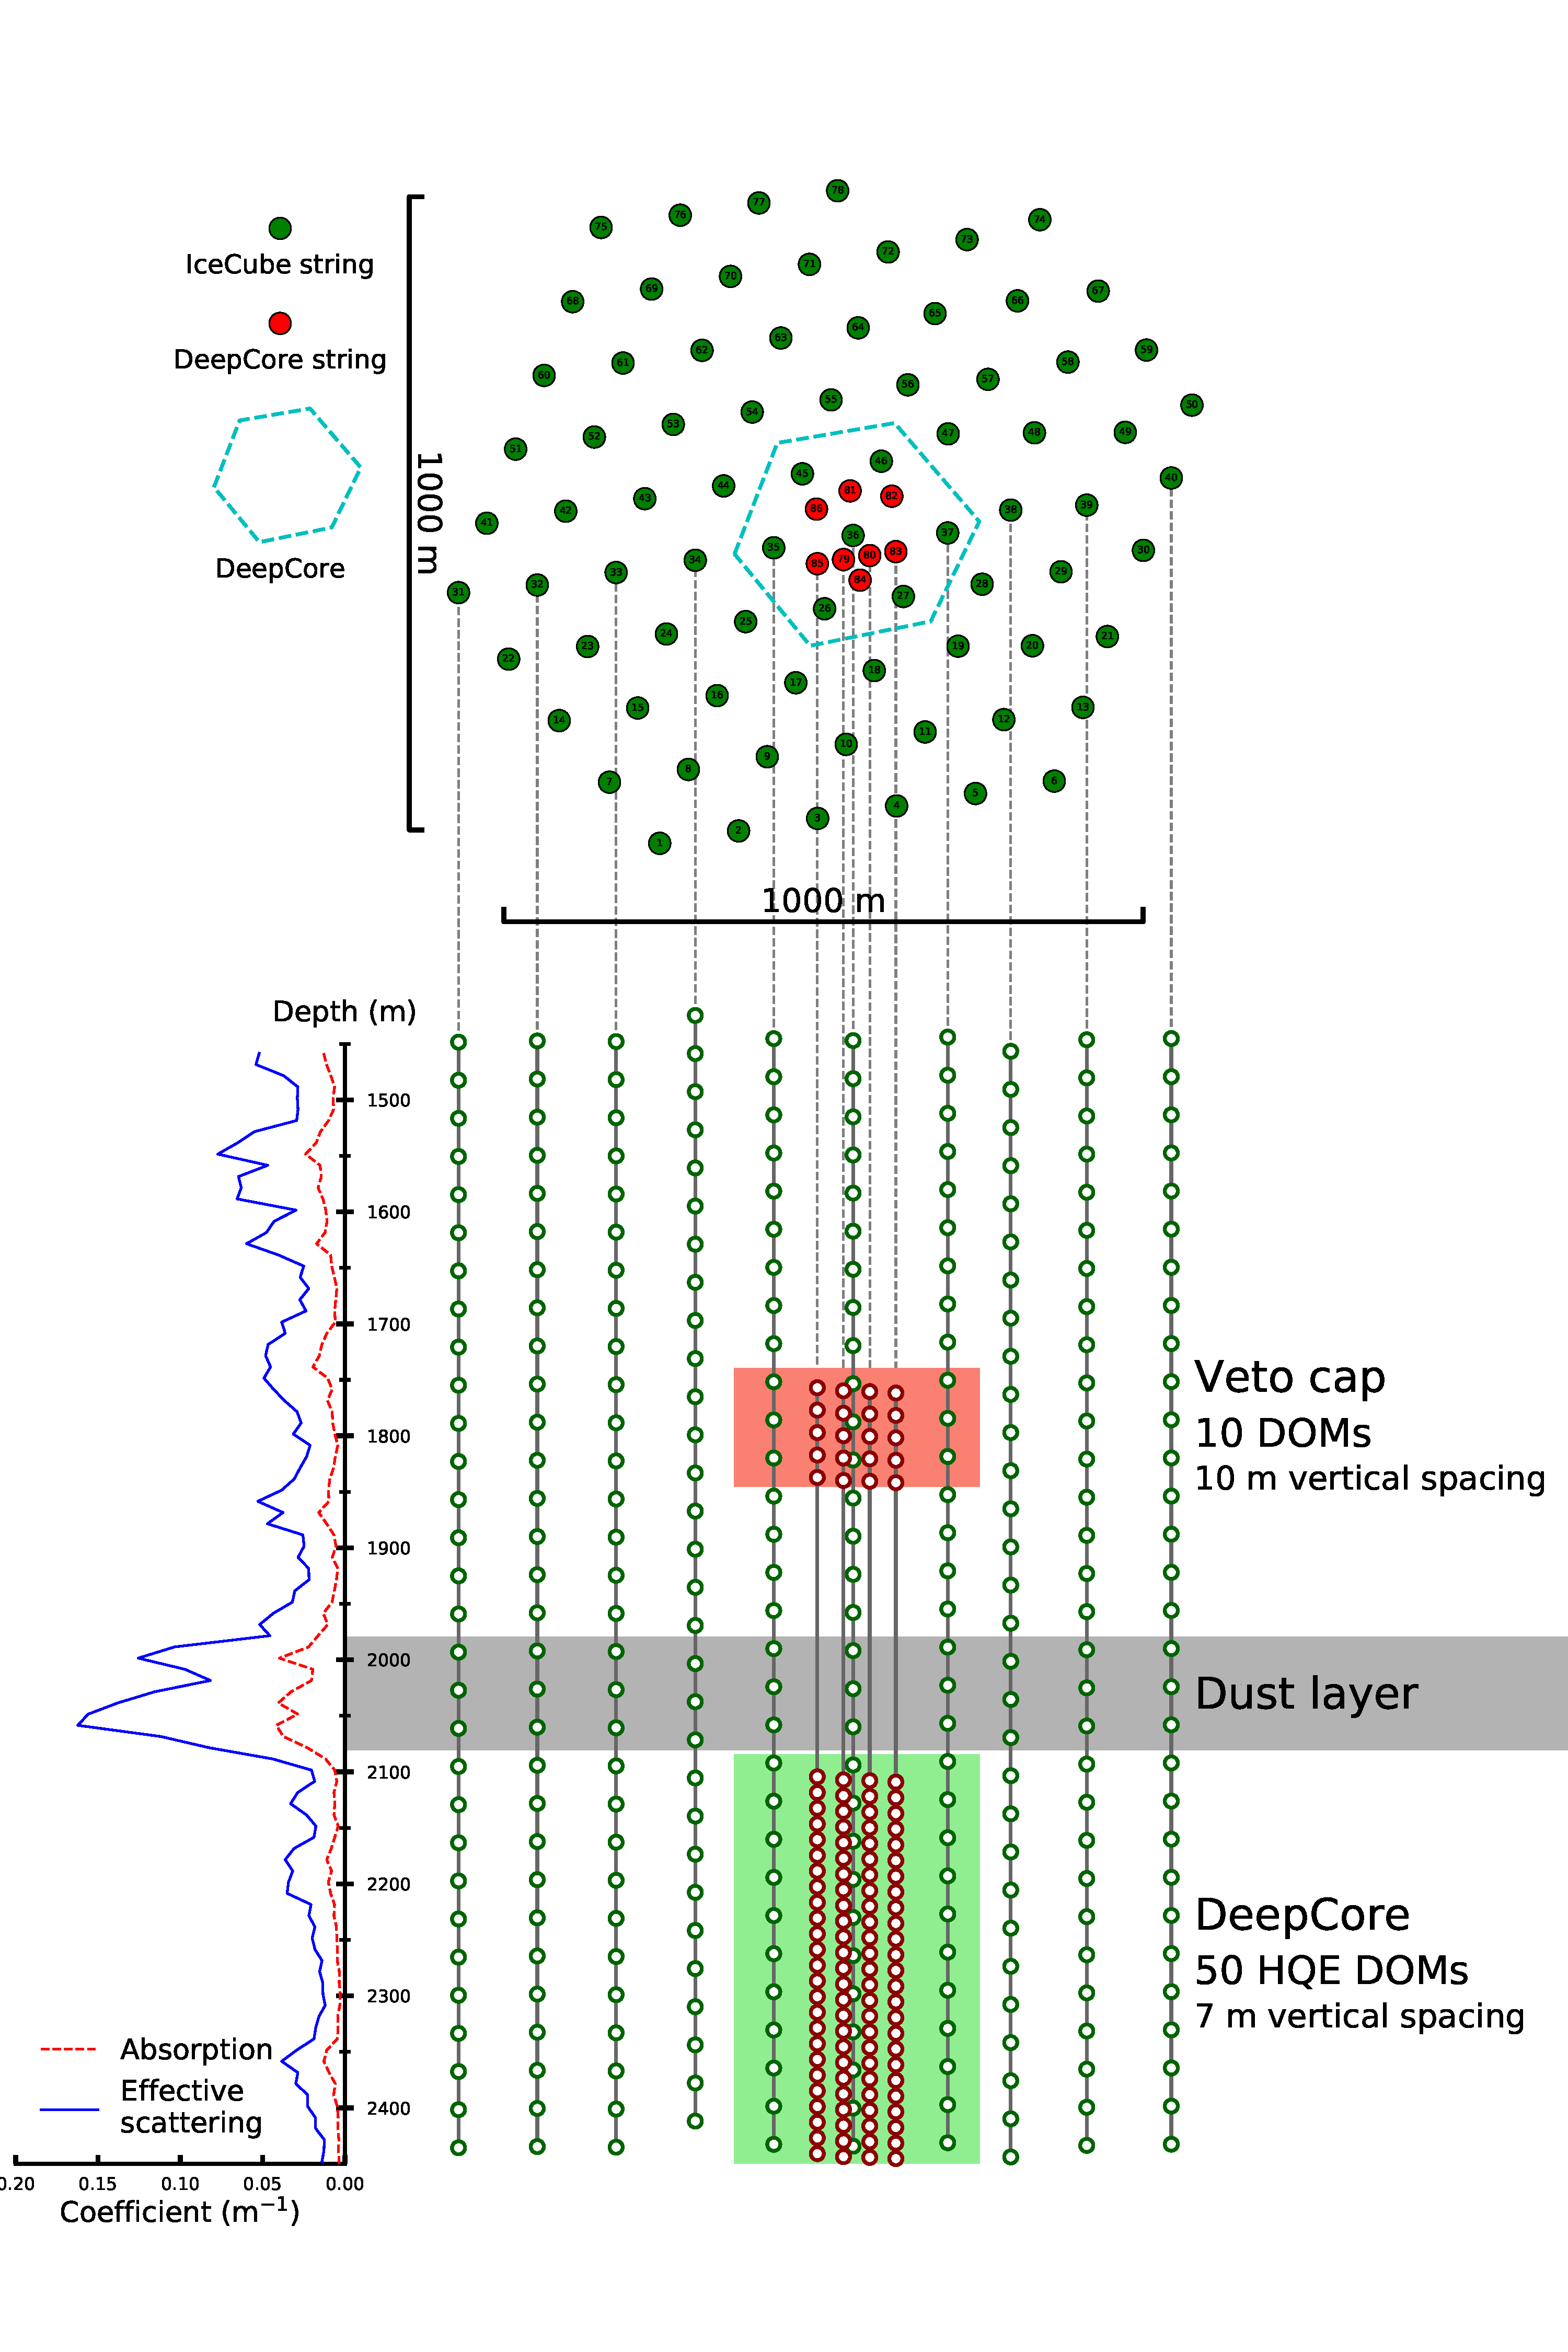
\includegraphics[width=0.9\linewidth]{figures/icecube/DeepCore_geometry.pdf}
    \caption{Schematic view of the IceCube detector as seen from the top (upper panel) and the side(lower panel). The DeepCore fiducial volume is indicated by the hexagon in the upper panel and the green shaded area in the bottom panel. The side-band on the lower panel shows the scattering and absorption coefficients as a function of depth.}
    \label{fig:icecube-schematic}
\end{figure}

\subsection{IceTop}

In addition to the in-ice array, IceCube also contains a surface array called \emph{IceTop}, consisting of 81 stations spread across an area of 1~km$^2$ that is used to detect muons from air showers.
It is typically used as a veto against atmospheric muons, but also functions as a detector in its own right measuring the spectrum and composition of cosmic particles.
%TODO: citation
However, it is not relevant to the measurement presented in this thesis.

\subsection{Digital Optical Modules}
\label{sec:dom-daq}
The Cherenkov radiation produced by charged particles in the ice is detected and digitized by Digital Optical Modules (DOMs).
Each module consists of a photo-multiplier tube (PMT)\sidecite{Abbasi_2010} and electronics housed in a transparent, spherical glass vessel that can withstand the enormous pressure below a water column of 2.5~km\cite{icecube_detector_17}.
They are each held in place by a harness attached to chains that allows the string cable to pass beside the DOM as shown in \reffig{dom-cable-assembly}.
\begin{marginfigure}[*-20]
    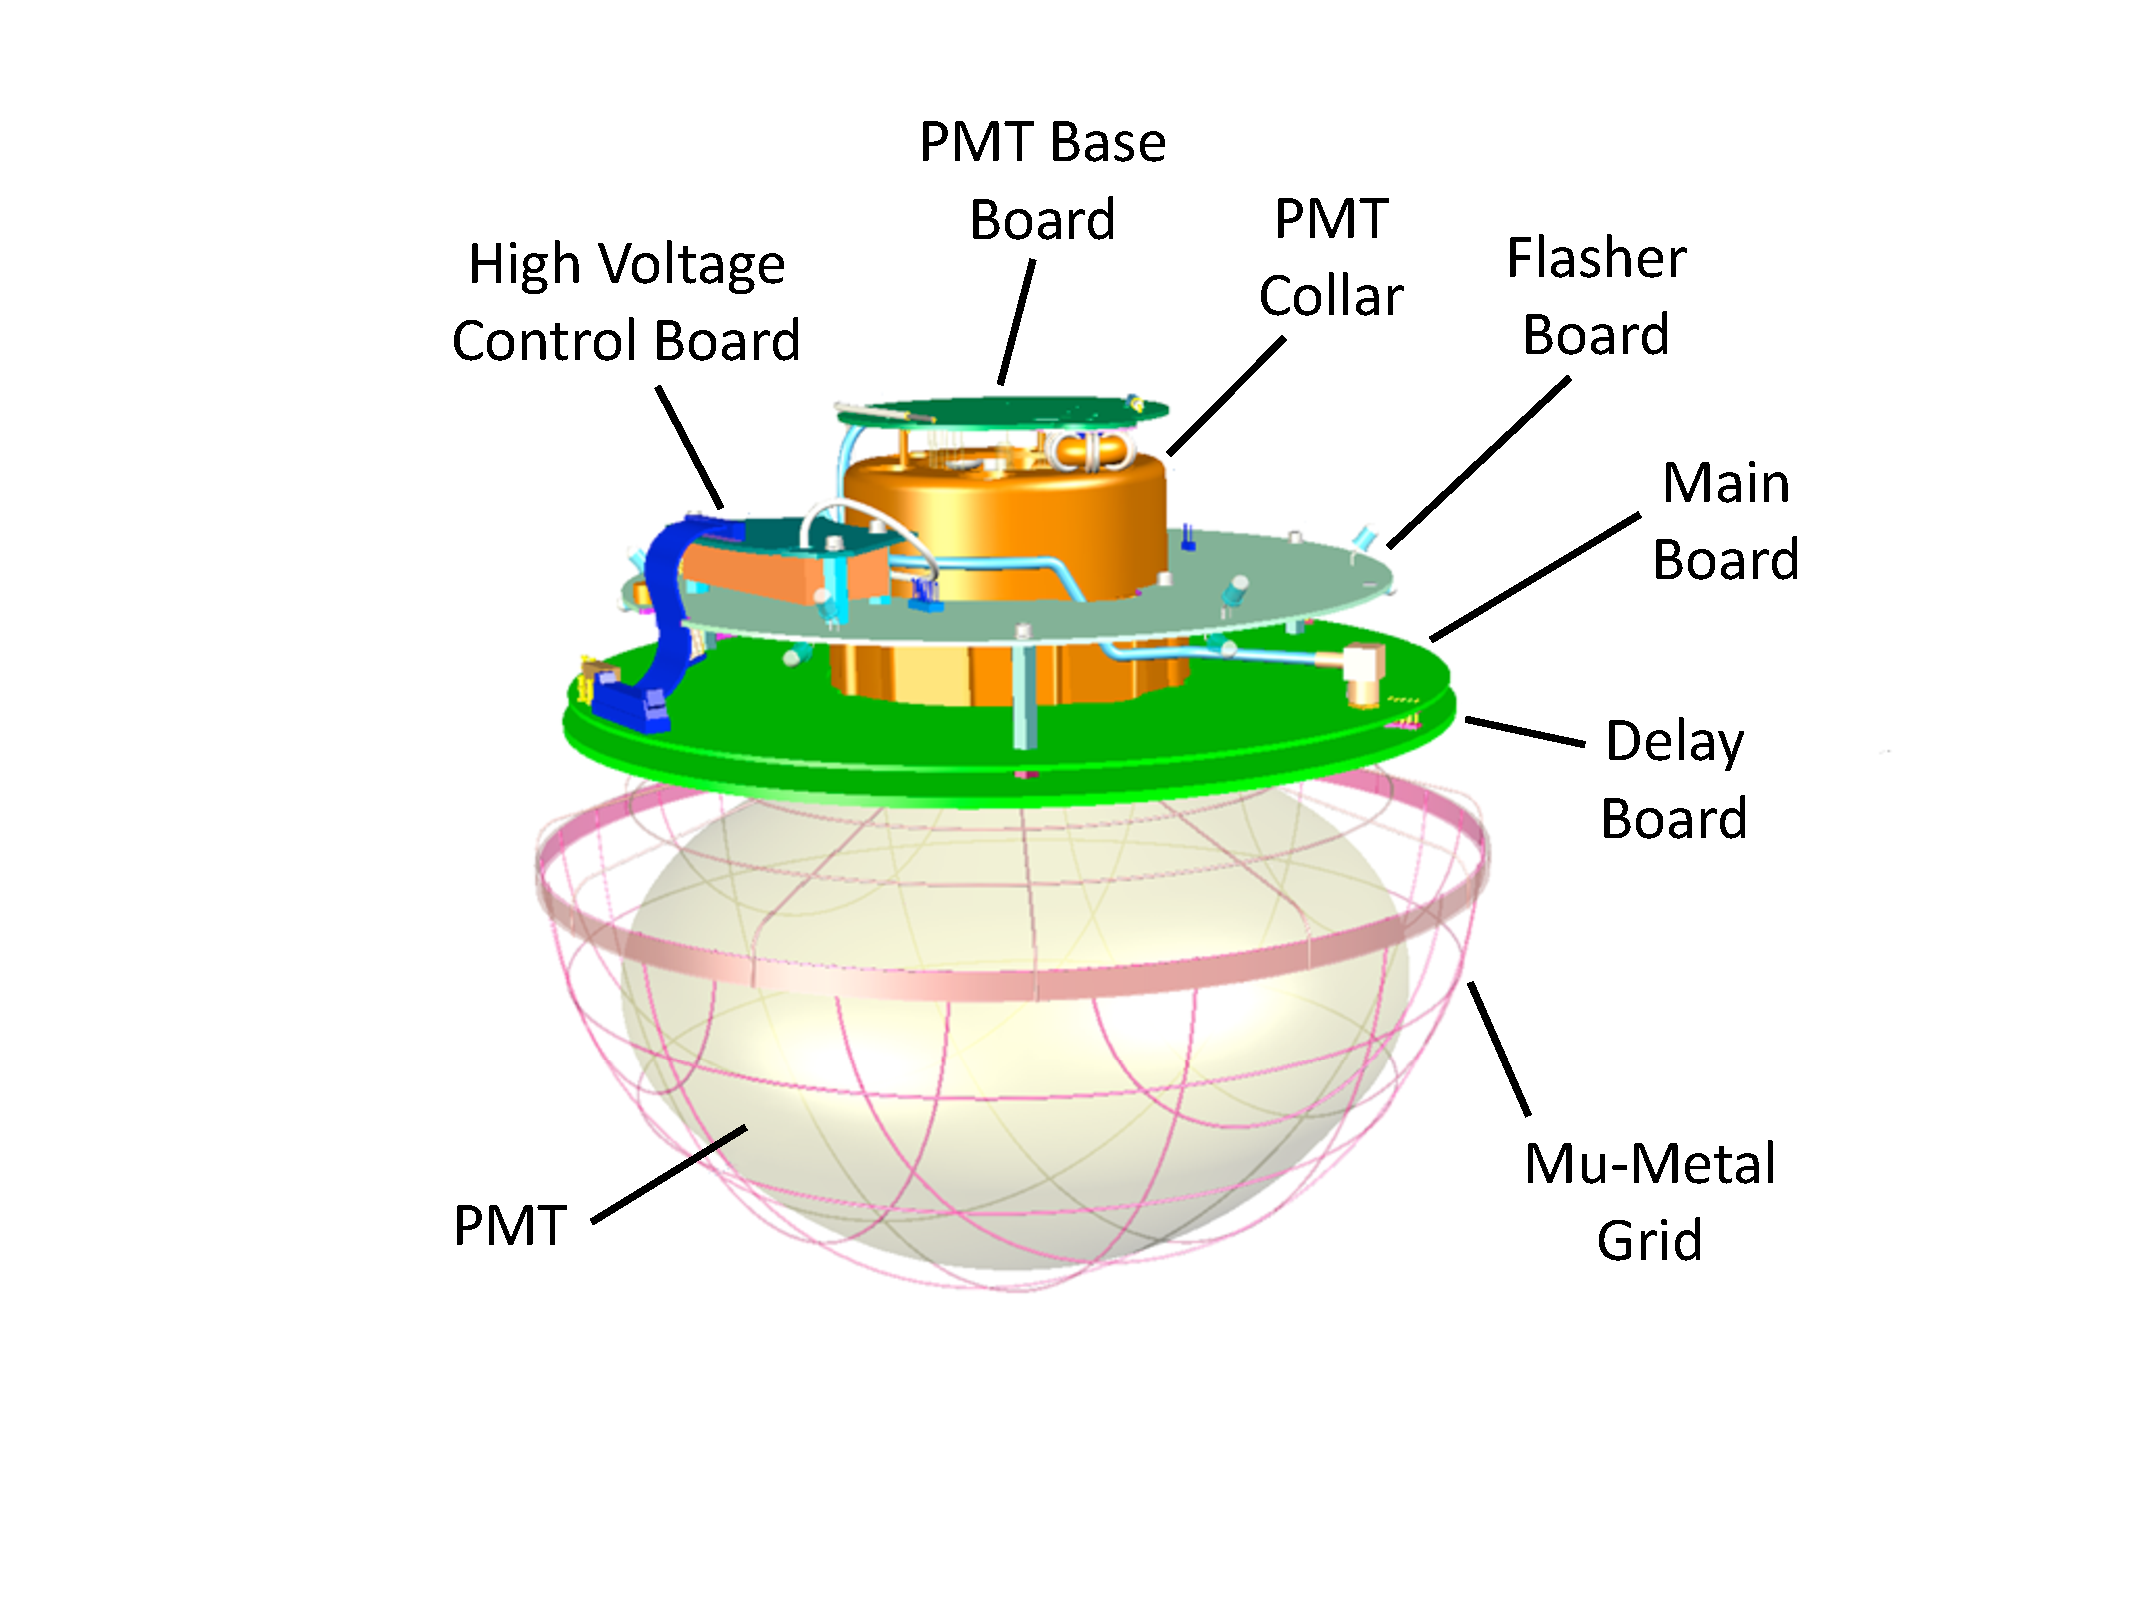
\includegraphics[width=\textwidth]{figures/icecube/domfig1a-DOM3DModel.pdf}
    \caption{Schematic of a DOM, taken from \cite{icecube_detector_17}.}
    \label{fig:dom-schematic}
\end{marginfigure}
\begin{marginfigure}
    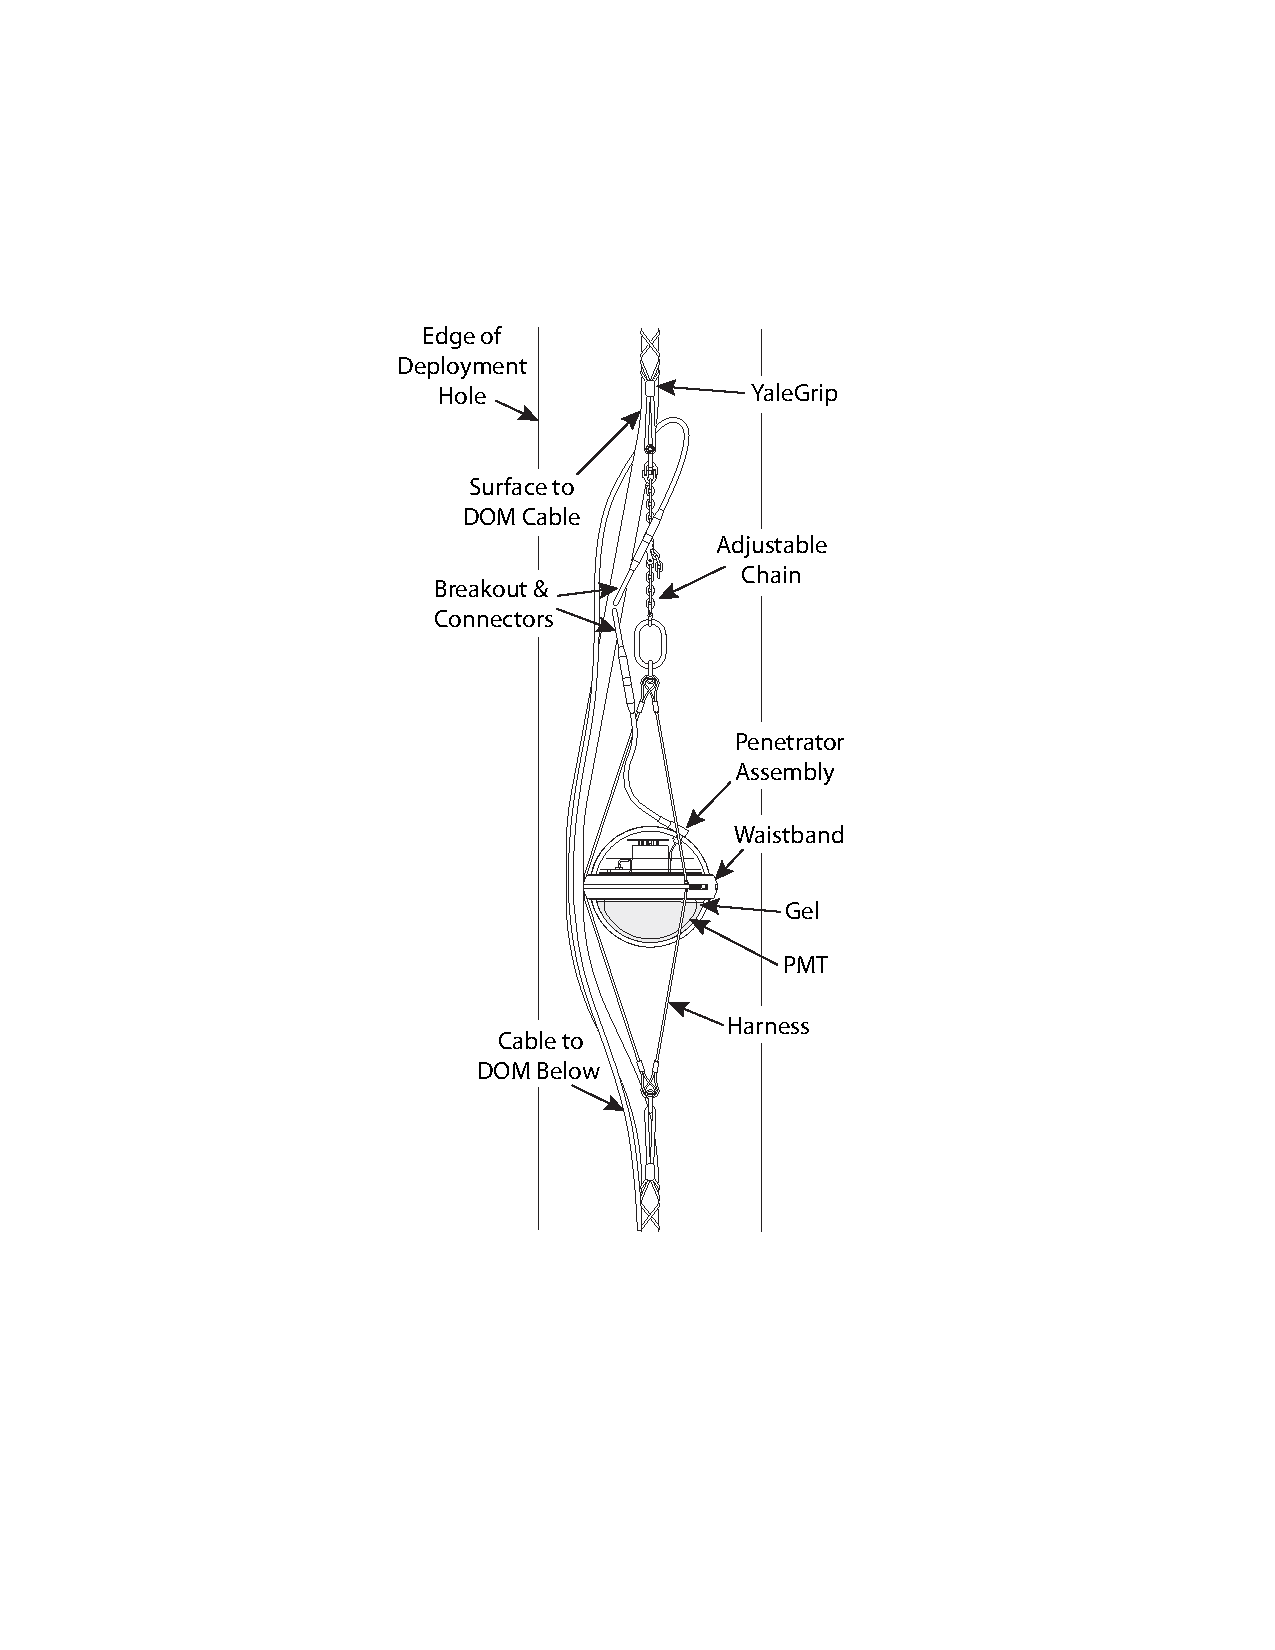
\includegraphics[width=\textwidth]{figures/icecube/domfig2a-CableAssembly.pdf}
    \caption{Schematic of the cable assembly of a DOM. Figure taken from \cite{icecube_detector_17}.}
    \label{fig:dom-cable-assembly}
\end{marginfigure}
The PMTs have a diameter of 10 inches and are sensitive to photons with wavelengths between 300~nm and 650~nm, with a maximum quantum efficiency of about 25\% at 390~nm.
Inside the DeepCore array, the peak efficiency reaches 34\%.
They are shielded from external magnetic fields with a mu-metal grid as shown in the schematic in Figure~\ref{fig:dom-schematic}.
The voltage at the PMT is measured and digitized by the on-board electronics\sidecite{icecube_daq} of the DOM in two separate readouts that are activated when the measured voltage rises above the equivalent of 0.25 photo-electrons (PE).
The first readout is the \emph{fast Analog-Digital Converter (fADC)} and measures the waveform continuously at a rate of 40~MHz.
The second readout, the \emph{Analog Transient Waveform Digitizer (ATWD)}, records the PMT voltage at a rate of 300~MHz in three channels with different gain levels to ensure that a large range\todo{what range?} of voltages can be recorded without saturation of the output.
The readout frequency of the ATWD is too high to be directly digitized and sent to the surface.
Instead, the ATWD voltage readout is buffered in 128 analog capacitors, corresponding to a readout time of $\sim$420~ns.
The buffered voltages are only digitized when at least one of the nearest or next-to-nearest DOMs on the same string also measures a signal within a 1~$\mu$s time window, which is referred to as the \emph{hard local coincidence (HLC)} condition.
The recorded waveforms are sent to the ICL on the surface, where they are compressed by applying the \emph{wavedeform} algorithm\sidecite{ic_spe_20}.
The output of this algorithm are reconstructed times and charges of single photo-electrons, which are taken as input by all further data processing steps described in section~\ref{sec:data-processing}.

The DOMs also contain a flasher board with 12 LEDs that can be used to emit pulsed light for the purpose of \emph{in-situ} detector calibration during special \emph{flasher runs} of the detector.
During such runs, the charge and time distributions of the observed pulses in the DOMs in response to the LED flashes are measured.
Since the light is emitted at known locations and at known times, the measured distributions allow inference on the absorption and scattering properties of the ice.
Because the total amplitude of the emitted light is less well known, this calibration method is less well suited for calibrating the total optical efficiency of the DOMs.
Instead, this property of the detector is calibrated more accurately from measurements of minimally-ionizing atmospheric muons, for which the energy loss is well known.


\section{Propagation of particles in ice}
\label{sec:particle-interactions}
Neutrinos interacting with the ice mostly interact via Deep Inelastic Scattering (DIS), creating muons, electromagnetic showers, and hadronic showers, depending on the flavor of the neutrino and interaction type.
The secondary particles produced by those interactions travel through the ice at highly relativistic velocities and lose energy primarily through ionization, bremsstrahlung, pair production and photo-nuclear interactions.
The fraction that each of these mechanisms contributes to the total energy loss of the particle depends on the type of particle and its energy.
When they are electrically charged, they also give off Cherenkov radiation that is then measured by IceCube.

\subsection{Cherenkov Effect}

The IceCube Neutrino Observatory relies entirely on the Cherenkov effect\sidecite{PhysRev.52.378} to detect particle interactions.
It is created by any electrically charged particle travelling through a transparent medium with velocities faster than the speed of light in that medium, $c/n$, where $n$ is the refractive index of the medium.
This produces a cone of light moving with the particle similar to a super-sonic shock that is generated by an object travelling through a gas at a velocity above the speed of sound.
The effect can be most easily understood according to Huygen's principle as a superposition of spherical light emissions that are produced every time that the particle displaces the charges in the dielectric medium in its closest vicinity, as shown in Figure~\ref{fig:cherenkov-sketch}.
When the particle is over-taking its own light emissions, they overlap coherently and form a conical light front as illustrated in the bottom panel of Figure~\ref{fig:cherenkov-sketch}.
\begin{marginfigure}[*-20]
    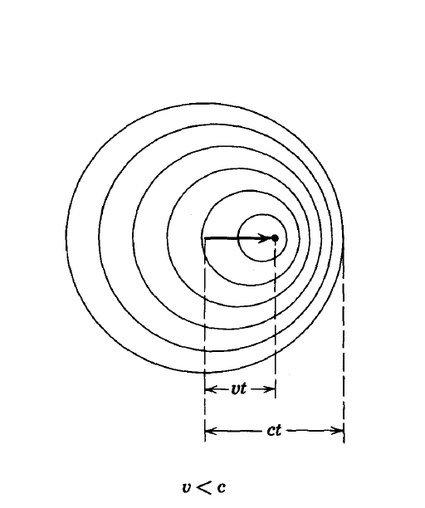
\includegraphics[width=\textwidth]{figures/icecube/cherenkov/cherenkov_slow.jpeg}
    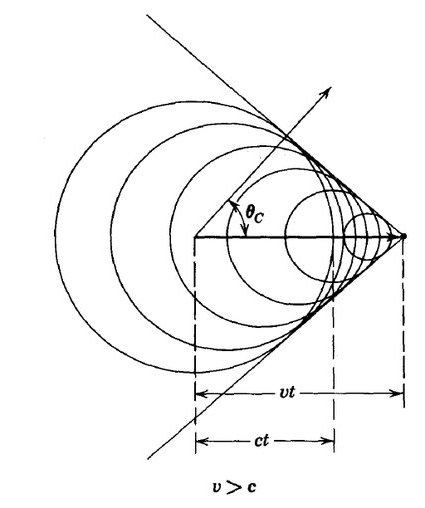
\includegraphics[width=\textwidth]{figures/icecube/cherenkov/cherenkov_fast.jpeg}
    \caption{An electrically charged particle emitting light while travelling below (upper panel) and above (lower panel) the speed of light in a medium. Image taken from \cite{jackson2012classical}.}
    \label{fig:cherenkov-sketch}
\end{marginfigure}
When the velocity of the particle is very close to the speed of light, as is the case for all (known) particles observable by IceCube, the opening angle of the cone only depends on the refractive index of the medium with
\begin{equation}
    \cos(\vartheta_c)=\frac{1}{\beta n}\;,
\end{equation}
where $n$ is the index of refraction and $\vartheta_c$ is the Cherenkov opening angle.

The frequency spectrum of the Cherenkov emissions of highly relativistic particles depends only on the charge of the particle, $q$, and the (wavelength-dependent) index of refraction, $n(\omega)$, and permeability, $\mu(\omega)$, of the medium.
The emitted energy per unit of distance and frequency is given by the Frank-Tamm-Equation\sidecite{Frank1937CoherentVR}\sidecite{Tamm1991}, which simplifies in the case of $v\approx c$ to
\begin{equation}
    \frac{\drm E}{\drm x \drm \omega}=\frac{q^2}{4\pi}\mu(\omega)\omega\left(1-\frac{1}{n^2(\omega)}\right)\,.
\end{equation}
The equation shows that the intensity of the Cherenkov emission generally increases with frequency, and indeed the strongest emissions are in the ultraviolet part of the spectrum.

\subsection{Muons}
\label{sec:muon-propagation}
At energies below 100~GeV, the dominant energy loss for muons is via ionization, and has only a weak dependence on energy.
Because the ionization loss is continuous and nearly constant, muons at these energies produce long, track-like signatures in the detector.
Above 100~GeV, the losses due to bremsstrahlung, pair production and photo-nuclear interactinos rise quickly in their amplitude and become dominant over ionization at $\sim$1~TeV.
The total average energy loss per unit distance, $\left<\drm E/\drm x\right>$, can be approximated combining all radiative energy losses (i.e.
all losses except for ionization) into one component and adding it to the ionization loss such that
\begin{equation}
    \left<-\frac{\drm E}{\drm x}\right> = a_I(E) + b_R(E)E\,,
\end{equation}
where $a_I(E)$ and $b_R(E)$ are slowly changing functions describing the ionization loss and the radiative losses, respectively\cite{muonstoppingpower}. For the energy ranges relevant for this work, the energy dependence of $a_I(E)$ and $b_R(E)$ is weak enough such that they can be approximated as constant numbers with $a_I(E)\approx 2\;\mathrm{MeV/cm}$ and $b_R(E)\approx3.4\times10^{-6}\;\mathrm{cm^{-1}}$\cite{muonstoppingpower}.
In this approximation, we can calculate the average length of a muon track, $\left<L\right>$, as a function of energy with
\begin{equation}
    \left<L\right>=\frac{1}{b_R}\log\left(\frac{b_R}{a_I}E + 1\right)\,,
\end{equation}
which gives an average travel distance of 50~m at 10~GeV and 460~m at 100~GeV.

\subsection{Electromagnetic Showers}
\label{sec:em-showers}
In contrast to muons, electrons and positrons lose their energy very quickly by emitting highly energetic photons due to bremsstrahlung.
The energy of the emitted photons is high enough that they spontaneously produce pairs of electrons and positrons.
This process is repeated until the electrons and positrons reach their critical energy, which is approximately 78~MeV in ice\sidecite{pdg}.
Below the critical energy, ionization takes over as the predominant mechanism of energy loss, which produces no new shower particles.
Another important quantity is the \emph{radiation length}, $X_0$, defined as the distance at which the energy of an electron is reduced to $\nicefrac{1}{e}$ of its initial energy via bremsstrahlung, which is 36~cm in ice\cite{pdg}.
The radiation length also determines the scale of the longitudinal development of the shower.
Expressing distances in units of radiation length as $t=x/X_0$, the shower intensity follows roughly a gamma distribution parametrized as
\begin{equation}
    \frac{\drm E}{\drm t} = E_0 b \frac{(bt)^{a-1}e^{-bt}}{\Gamma(a)}\;,
\end{equation}
where the parameters $a$ and $b$ need to be fit empirically\cite{pdg}.
Their values for electrons, positrons and photons interacting in ice have been determined from GEANT4\sidecite{geant4} shower simulations in\sidecite{RADEL2013102} to be
\begin{subequations}\label{eq:shower-params}
\begin{align}
    a &\approx 2.01 + 1.46 \log_{10}(E_0/\mathrm{GeV}),\; b\approx 0.63\; & (e^+,e^-), \label{eq:shower-params-1}\\
    a &\approx 2.84 + 1.34 \log_{10}(E_0/\mathrm{GeV}),\; b\approx 0.65\; & (\gamma).\label{eq:shower-params-2}
\end{align}
\end{subequations}
The shower reaches its maximum intensity at a distance of
\begin{equation}
    t_{\mathrm{max}}=\frac{a-1}{b}\;,
\end{equation}
which corresponds to a logarithmic growth of the size of the cascade according to \cref{eq:shower-params-1,eq:shower-params-2}.
The electrically charged components of the electromagnetic shower produce Cherenkov light, where the emissions peak at the Cherenkov angle since the secondary particles are emitted very close to the forward direction as shown in \reffig{cherenkov_angular_profile_cascade}.

\begin{marginfigure}
    \centering
    \tikzsetnextfilename{cascade_cherenkov_angular_dist}%
    % This file was created with tikzplotlib v0.10.1.
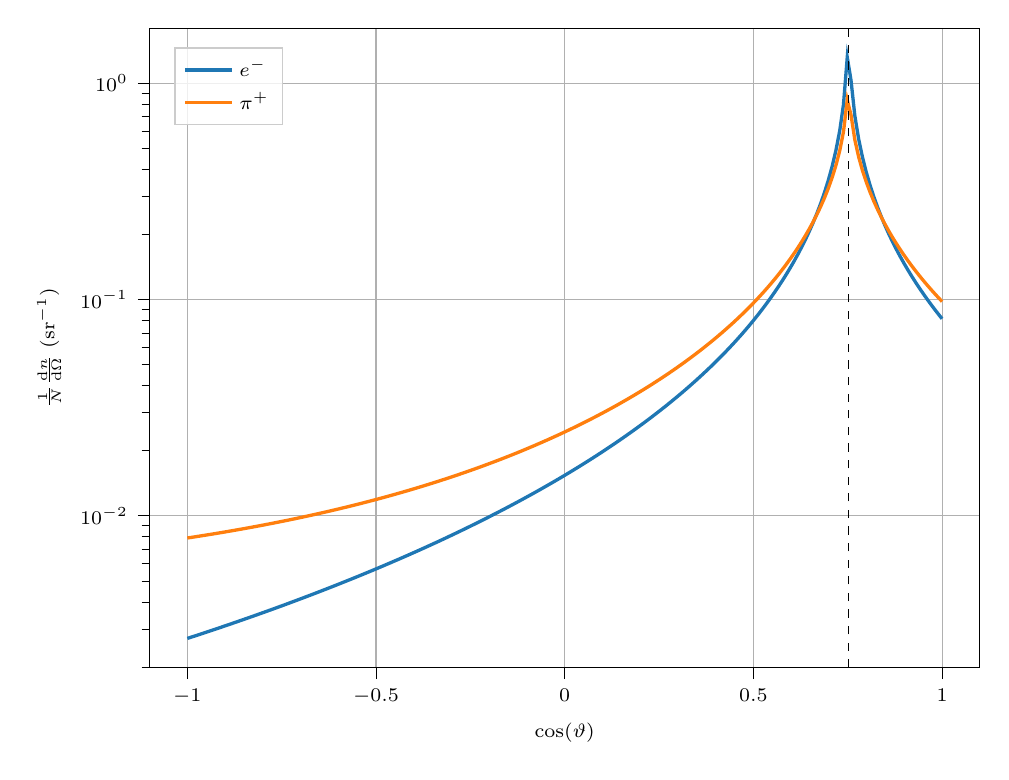
\begin{tikzpicture}

\definecolor{darkgray176}{RGB}{176,176,176}
\definecolor{darkorange25512714}{RGB}{255,127,14}
\definecolor{lightgray204}{RGB}{204,204,204}
\definecolor{steelblue31119180}{RGB}{31,119,180}

\begin{axis}[
height=0.8\linewidth,
legend cell align={left},
legend style={
  fill opacity=0.8,
  draw opacity=1,
  text opacity=1,
  at={(0.03,0.97)},
  anchor=north west,
  draw=lightgray204
},
log basis y={10},
minor xtick={},
minor ytick={0.0002,0.0003,0.0004,0.0005,0.0006,0.0007,0.0008,0.0009,0.002,0.003,0.004,0.005,0.006,0.007,0.008,0.009,0.02,0.03,0.04,0.05,0.06,0.07,0.08,0.09,0.2,0.3,0.4,0.5,0.6,0.7,0.8,0.9,2,3,4,5,6,7,8,9,20,30,40,50,60,70,80,90,200,300,400,500,600,700,800,900},
tick align=outside,
tick pos=left,
width=\linewidth,
x grid style={darkgray176},
xlabel={\(\scriptstyle \cos(\vartheta)\)},
xmajorgrids,
xmin=-1.1, xmax=1.1,
xtick style={color=black},
xtick={-1.5,-1,-0.5,0,0.5,1,1.5},
xticklabels={
\(\scriptstyle -1.5\),
\(\scriptstyle -1\),
\(\scriptstyle -0.5\),
\(\scriptstyle 0\),
\(\scriptstyle 0.5\),
\(\scriptstyle 1\),
\(\scriptstyle 1.5\)
},
y grid style={darkgray176},
ylabel={\(\scriptstyle \frac{1}{N}\frac{\mathrm{d}n}{\mathrm{d}\Omega}\;(\mathrm{sr^{-1}})\)},
ymajorgrids,
ymin=0.00198893054244642, ymax=1.79304902414132,
ymode=log,
ytick style={color=black},
ytick={0.0001,0.001,0.01,0.1,1,10,100},
yticklabels={
  \(\scriptstyle {10^{-4}}\),
  \(\scriptstyle {10^{-3}}\),
  \(\scriptstyle {10^{-2}}\),
  \(\scriptstyle {10^{-1}}\),
  \(\scriptstyle {10^{0}}\),
  \(\scriptstyle {10^{1}}\),
  \(\scriptstyle {10^{2}}\)
}
]
% \addlegendimage{empty legend}
% \addlegendentry{\hspace{-.6cm}\(\scriptstyle Primary particle\)}
\addplot [very thick, steelblue31119180]
table {%
-1 0.00270979570996691
-0.989949748743719 0.00274568176844791
-0.979899497487437 0.00278221344276632
-0.969849246231156 0.0028194051401974
-0.959798994974874 0.00285727165740652
-0.949748743718593 0.00289582819293
-0.939698492462312 0.002935090360122
-0.92964824120603 0.00297507420058719
-0.919597989949749 0.00301579619812029
-0.909547738693467 0.00305727329317443
-0.899497487437186 0.00309952289788118
-0.889447236180904 0.00314256291164658
-0.879396984924623 0.00318641173734847
-0.869346733668342 0.00323108829816169
-0.85929648241206 0.00327661205503912
-0.849246231155779 0.00332300302487796
-0.839195979899497 0.00337028179940208
-0.829145728643216 0.00341846956479283
-0.819095477386935 0.00346758812210248
-0.809045226130653 0.00351765990848599
-0.798994974874372 0.00356870801928906
-0.78894472361809 0.00362075623103195
-0.778894472361809 0.00367382902533086
-0.768844221105528 0.00372795161380099
-0.758793969849246 0.00378314996398742
-0.748743718592965 0.00383945082637282
-0.738693467336683 0.00389688176251318
-0.728643216080402 0.00395547117435602
-0.718592964824121 0.00401524833479813
-0.708542713567839 0.00407624341954317
-0.698492462311558 0.00413848754032286
-0.688442211055276 0.00420201277954891
-0.678391959798995 0.00426685222646659
-0.668341708542714 0.00433304001488506
-0.658291457286432 0.00440061136256355
-0.648241206030151 0.00446960261233712
-0.638190954773869 0.00454005127507061
-0.628140703517588 0.00461199607453446
-0.618090452261307 0.00468547699430147
-0.608040201005025 0.00476053532676948
-0.597989949748744 0.0048372137244211
-0.587939698492462 0.00491555625343831
-0.577889447236181 0.00499560844979658
-0.5678391959799 0.00507741737797107
-0.557788944723618 0.00516103169239503
-0.547738693467337 0.00524650170181962
-0.537688442211055 0.00533387943673301
-0.527638190954774 0.0054232187200069
-0.517587939698492 0.00551457524094897
-0.507537688442211 0.0056080066329506
-0.49748743718593 0.00570357255493209
-0.487437185929648 0.00580133477679948
-0.477386934673367 0.00590135726914189
-0.467336683417085 0.00600370629741217
-0.457286432160804 0.0061084505208506
-0.447236180904523 0.00621566109642723
-0.437185929648241 0.00632541178809819
-0.42713567839196 0.00643777908168967
-0.417085427135678 0.00655284230574558
-0.407035175879397 0.00667068375869704
-0.396984924623116 0.00679138884273666
-0.386934673366834 0.00691504620480722
-0.376884422110553 0.00704174788514251
-0.366834170854271 0.00717158947382927
-0.35678391959799 0.00730467027589214
-0.346733668341708 0.0074410934854396
-0.336683417085427 0.00758096636944745
-0.326633165829146 0.0077244004617986
-0.316582914572864 0.00787151176824312
-0.306532663316583 0.0080224209829917
-0.296482412060301 0.00817725371770887
-0.28643216080402 0.00833614074373032
-0.276381909547739 0.00849921824839105
-0.266331658291457 0.00866662810641917
-0.256281407035176 0.0088385181674243
-0.246231155778894 0.00901504256058975
-0.236180904522613 0.00919636201776539
-0.226130653266332 0.00938264421625311
-0.21608040201005 0.0095740641426814
-0.206030150753769 0.00977080447947795
-0.195979899497487 0.00997305601557417
-0.185929648241206 0.0101810180831098
-0.175879396984925 0.0103948990220547
-0.165829145728643 0.0106149166748261
-0.155778894472362 0.0108412989131575
-0.14572864321608 0.0110742841996714
-0.135678391959799 0.0113141221868181
-0.125628140703518 0.0115610743560839
-0.115577889447236 0.0118154147006228
-0.105527638190955 0.0120774304547576
-0.0954773869346733 0.0123474228741045
-0.085427135678392 0.0126257080704248
-0.0753768844221105 0.0129126179056865
-0.0653266331658291 0.0132085009502441
-0.0552763819095478 0.0135137235105104
-0.0452261306532663 0.0138286707320131
-0.035175879396985 0.0141537477843051
-0.0251256281407035 0.0144893811348354
-0.0150753768844221 0.0148360199195975
-0.00502512562814073 0.0151941374191663
0.00502512562814061 0.0155642326496143
0.0150753768844221 0.0159468320787846
0.0251256281407035 0.0163424914795012
0.035175879396985 0.0167517979325291
0.0452261306532664 0.0171753719934818
0.0552763819095476 0.0176138700394269
0.0653266331658291 0.0180679868126891
0.0753768844221105 0.0185384581813153
0.085427135678392 0.0190260641378932
0.0954773869346734 0.0195316320609182
0.105527638190955 0.0200560402657496
0.115577889447236 0.0206002218754172
0.125628140703518 0.0211651690451993
0.135678391959799 0.0217519375790622
0.14572864321608 0.022361651980798
0.155778894472362 0.0229955109881295
0.165829145728643 0.0236547936442626
0.175879396984925 0.0243408659685004
0.185929648241206 0.0250551882957267
0.195979899497488 0.0257993233640178
0.206030150753769 0.0265749452405507
0.21608040201005 0.0273838491886102
0.226130653266332 0.0282279625931581
0.236180904522613 0.0291093570794933
0.246231155778895 0.0300302619794334
0.256281407035176 0.030993079322741
0.266331658291457 0.03200040055884
0.276381909547739 0.0330550252460245
0.28643216080402 0.0341599819833132
0.296482412060302 0.0353185519050526
0.306532663316583 0.0365342951117703
0.316582914572864 0.0378110804744502
0.326633165829146 0.0391531193255863
0.336683417085427 0.040565003641884
0.346733668341709 0.0420517494338256
0.35678391959799 0.0436188461909371
0.366834170854271 0.0452723133940923
0.376884422110553 0.0470187653046993
0.386934673366834 0.0488654854842812
0.396984924623116 0.0508205127985405
0.407035175879397 0.0528927410327426
0.417085427135678 0.055092034710039
0.42713567839196 0.057429364287307
0.437185929648241 0.0599169646387465
0.447236180904523 0.0625685216719253
0.457286432160804 0.0653993931161115
0.467336683417085 0.0684268710625494
0.477386934673367 0.0716704958356979
0.487437185929648 0.0751524333921324
0.49748743718593 0.0788979319015025
0.507537688442211 0.0829358777746636
0.517587939698493 0.0872994776151978
0.527638190954774 0.0920271010294813
0.537688442211055 0.0971633308874874
0.547738693467337 0.102760283897193
0.557788944723618 0.108879287382879
0.5678391959799 0.115593031243989
0.577889447236181 0.122988362403445
0.587939698492462 0.131169960953129
0.597989949748744 0.140265246331153
0.608040201005025 0.15043103123486
0.618090452261307 0.16186271048248
0.628140703517588 0.17480721310861
0.638190954773869 0.189581691206729
0.648241206030151 0.20660122497593
0.658291457286432 0.226421210798552
0.668341708542714 0.249804685334967
0.678391959798995 0.277834184784676
0.688442211055276 0.312108201800071
0.698492462311558 0.355111292696392
0.708542713567839 0.410978453421262
0.718592964824121 0.487286890541685
0.728643216080402 0.60012697327905
0.738693467336683 0.793910321136359
0.748743718592965 1.3160586073339
0.758793969849246 1.02808069276863
0.768844221105528 0.705773104929006
0.778894472361809 0.551690720919282
0.78894472361809 0.455470028921774
0.798994974874372 0.388094231142621
0.809045226130653 0.337707570767511
0.819095477386935 0.298358445355108
0.829145728643216 0.266664676520879
0.839195979899497 0.240535857090921
0.849246231155779 0.218598677952748
0.85929648241206 0.199907969806359
0.869346733668342 0.183788893273284
0.879396984924623 0.169745057977341
0.889447236180904 0.157402218673429
0.899497487437186 0.146472295437764
0.909547738693467 0.13672956196271
0.919597989949749 0.127994411299455
0.92964824120603 0.120122001115478
0.939698492462312 0.112994133285036
0.949748743718593 0.106513332049104
0.959798994974874 0.100598450200823
0.969849246231156 0.0951813583735468
0.979899497487437 0.090204415681687
0.989949748743719 0.0856185130166524
1 0.0813815420878193
};
\addlegendentry{\(\scriptstyle e^-\)}
\addplot [very thick, darkorange25512714]
table {%
-1 0.00789216051649666
-0.989949748743719 0.00794087635636688
-0.979899497487437 0.00799046060080033
-0.969849246231156 0.00804093213801919
-0.959798994974874 0.00809231034956343
-0.949748743718593 0.00814461512551476
-0.939698492462312 0.00819786688026744
-0.92964824120603 0.00825208656886829
-0.919597989949749 0.00830729570394975
-0.909547738693467 0.00836351637328043
-0.899497487437186 0.0084207712579593
-0.889447236180904 0.00847908365128039
-0.879396984924623 0.00853847747829651
-0.869346733668342 0.00859897731611185
-0.85929648241206 0.00866060841493438
-0.849246231155779 0.00872339671992113
-0.839195979899497 0.00878736889385044
-0.829145728643216 0.00885255234065718
-0.819095477386935 0.00891897522986894
-0.809045226130653 0.00898666652198258
-0.798994974874372 0.0090556559948231
-0.78894472361809 0.00912597427092828
-0.778894472361809 0.00919765284600533
-0.768844221105528 0.00927072411850768
-0.758793969849246 0.00934522142038275
-0.748743718592965 0.00942117904904423
-0.738693467336683 0.00949863230062473
-0.728643216080402 0.00957761750456841
-0.718592964824121 0.00965817205962519
-0.708542713567839 0.00974033447131266
-0.698492462311558 0.00982414439091419
-0.688442211055276 0.00990964265608621
-0.678391959798995 0.00999687133315109
-0.668341708542714 0.0100858737611565
-0.658291457286432 0.0101766945977864
-0.648241206030151 0.0102693798672131
-0.638190954773869 0.0103639770099861
-0.628140703517588 0.0104605349350563
-0.618090452261307 0.0105591040740432
-0.608040201005025 0.0106597364378548
-0.597989949748744 0.0107624856757796
-0.587939698492462 0.0108674071371743
-0.577889447236181 0.0109745579358802
-0.5678391959799 0.0110839970175068
-0.557788944723618 0.0111957852297315
-0.547738693467337 0.0113099853957697
-0.537688442211055 0.0114266623911839
-0.527638190954774 0.0115458832242044
-0.517587939698492 0.0116677171197494
-0.507537688442211 0.0117922356073411
-0.49748743718593 0.0119195126131274
-0.487437185929648 0.0120496245562312
-0.477386934673367 0.0121826504496634
-0.467336683417085 0.0123186720060495
-0.457286432160804 0.0124577737484374
-0.447236180904523 0.0126000431264682
-0.437185929648241 0.0127455706382125
-0.42713567839196 0.0128944499579918
-0.417085427135678 0.0130467780705269
-0.407035175879397 0.0132026554117768
-0.396984924623116 0.013362186016856
-0.386934673366834 0.0135254776754425
-0.376884422110553 0.0136926420951192
-0.366834170854271 0.0138637950731175
-0.35678391959799 0.0140390566769668
-0.346733668341708 0.0142185514345872
-0.336683417085427 0.0144024085343986
-0.326633165829146 0.0145907620360627
-0.316582914572864 0.0147837510925123
-0.306532663316583 0.0149815201839753
-0.296482412060301 0.0151842193647459
-0.28643216080402 0.0153920045235134
-0.276381909547739 0.0156050376581157
-0.266331658291457 0.0158234871656503
-0.256281407035176 0.0160475281489437
-0.246231155778894 0.0162773427404552
-0.236180904522613 0.0165131204447723
-0.226130653266332 0.0167550585009444
-0.21608040201005 0.0170033622659962
-0.206030150753769 0.0172582456210662
-0.195979899497487 0.0175199314017323
-0.185929648241206 0.0177886518542055
-0.175879396984925 0.0180646491192131
-0.165829145728643 0.0183481757455348
-0.155778894472362 0.0186394952353194
-0.14572864321608 0.0189388826234856
-0.135678391959799 0.0192466250936987
-0.125628140703518 0.0195630226336309
-0.115577889447236 0.0198883887324402
-0.105527638190955 0.0202230511236558
-0.0954773869346733 0.0205673525769393
-0.085427135678392 0.0209216517424914
-0.0753768844221105 0.0212863240522157
-0.0653266331658291 0.0216617626821167
-0.0552763819095478 0.0220483795808203
-0.0452261306532663 0.022446606569557
-0.035175879396985 0.0228568965194424
-0.0251256281407035 0.0232797246124452
-0.0150753768844221 0.0237155896930427
-0.00502512562814073 0.0241650157182394
0.00502512562814061 0.0246285533143807
0.0150753768844221 0.0251067814500269
0.0251256281407035 0.025600309235087
0.035175879396985 0.0261097778574502
0.0452261306532664 0.0266358626695118
0.0552763819095476 0.0271792754382893
0.0653266331658291 0.0277407667742745
0.0753768844221105 0.0283211287557975
0.085427135678392 0.0289211977675074
0.0954773869346734 0.0295418575736295
0.105527638190955 0.0301840426489816
0.115577889447236 0.0308487417933436
0.125628140703518 0.0315370020577348
0.135678391959799 0.032249933014505
0.14572864321608 0.032988711406942
0.155778894472362 0.0337545862184264
0.165829145728643 0.0345488842060796
0.175879396984925 0.0353730159494754
0.185929648241206 0.0362284824714063
0.195979899497488 0.0371168824950634
0.206030150753769 0.0380399204104475
0.21608040201005 0.0389994150325696
0.226130653266332 0.0399973092452438
0.236180904522613 0.0410356806372771
0.246231155778895 0.0421167532529549
0.256281407035176 0.0432429105962605
0.266331658291457 0.0444167100487352
0.276381909547739 0.0456408988848156
0.28643216080402 0.0469184320965592
0.296482412060302 0.048252492272703
0.306532663316583 0.0496465118159931
0.316582914572864 0.0511041978289106
0.326633165829146 0.0526295600528103
0.336683417085427 0.0542269423109717
0.346733668341709 0.0559010579844757
0.35678391959799 0.0576570301440859
0.366834170854271 0.0595004370751213
0.376884422110553 0.0614373640703005
0.386934673366834 0.0634744625336283
0.396984924623116 0.0656190176441357
0.407035175879397 0.0678790260813921
0.417085427135678 0.0702632856277359
0.42713567839196 0.0727814988515182
0.437185929648241 0.075444393562777
0.447236180904523 0.0782638633461016
0.457286432160804 0.0812531322528268
0.467336683417085 0.0844269487270227
0.477386934673367 0.0878018151159875
0.487437185929648 0.0913962607705643
0.49748743718593 0.0952311689042153
0.507537688442211 0.099330170235027
0.517587939698493 0.103720120240028
0.527638190954774 0.108431681976416
0.537688442211055 0.113500043406718
0.547738693467337 0.118965807795903
0.557788944723618 0.124876109212345
0.5678391959799 0.131286024264284
0.577889447236181 0.138260378736104
0.587939698492462 0.145876088183355
0.597989949748744 0.154225231976222
0.608040201005025 0.163419152664381
0.618090452261307 0.173594017226095
0.628140703517588 0.18491850963698
0.638190954773869 0.197604710766709
0.648241206030151 0.211923886477276
0.658291457286432 0.228230096197278
0.668341708542714 0.246996774450726
0.678391959798995 0.26887589872466
0.688442211055276 0.294798880744473
0.698492462311558 0.32616049150544
0.708542713567839 0.36518484083375
0.718592964824121 0.41574694864329
0.728643216080402 0.48557899814055
0.738693467336683 0.594309602959545
0.748743718592965 0.835983791833013
0.758793969849246 0.710693050136147
0.768844221105528 0.546432769731992
0.778894472361809 0.456265851073738
0.78894472361809 0.395022749599503
0.798994974874372 0.349420179510256
0.809045226130653 0.313615587438124
0.819095477386935 0.284503587518325
0.829145728643216 0.260234102069794
0.839195979899497 0.239616407766554
0.849246231155779 0.221839941214909
0.85929648241206 0.206328850988604
0.869346733668342 0.192660020219313
0.879396984924623 0.180513958673293
0.889447236180904 0.169643916401901
0.899497487437186 0.159855667085849
0.909547738693467 0.150993826949325
0.919597989949749 0.142932331066801
0.92964824120603 0.135567640702552
0.939698492462312 0.128813795145942
0.949748743718593 0.122598739772099
0.959798994974874 0.116861556117663
0.969849246231156 0.111550341625584
0.979899497487437 0.10662056525917
0.989949748743719 0.102033776999246
1 0.0977565841356766
};
\addlegendentry{\(\scriptstyle \pi^+\)}
\addplot [black, dashed, forget plot]
table {%
0.75187969924812 0.00198893054244642
0.75187969924812 1.79304902414132
};
\end{axis}

\end{tikzpicture}


    \caption{Angular profile of the Cherenkov emission of an electromagnetic cascade ($e^-$) and a hadronic cascade ($\pi^+$) using the parametrization from \cite{RADEL2013102}.}
    \label{fig:cherenkov_angular_profile_cascade}
\end{marginfigure}

\subsection{Hadronic Showers}
\label{sec:had-showers}
As discussed in section~\ref{sec:neutrino-xsec}, neutrino interactions above 10~GeV happen almost exclusively via Deep-Inelastic Scattering (DIS).
These interactions always produce a hadronic cascade in addition to any leptons in the final state.
Hadronic cascades are also the only visible part of the final state of neutral-current interactions.
Hadrons (mostly Pions) that are produced in neutrino-nucleon interactions interact strongly with the surrounding ice to create secondary particles and then decay to form additional photons and leptons.
Charged secondary particles produce Cherenkov radiation, while neutral secondary particles are invisible to the detector.
Because part of the energy deposited in a hadronic shower is not measurable, the inherent uncertainty on the true energy of the primary particle that initiated the interaction is larger.
The average visible electromagnetic fraction of a hadronic shower can be parametrized\cite{RADEL2013102} as a function of the initial energy with
\begin{equation}
    F(E_0) = 1 - (1-f_0)\left(\frac{E_0}{E_s}\right)^{-m}
\end{equation}
with a variance of
\begin{equation}
    \sigma_F(E_0) = \sigma_0 \log(E_0)^{-\gamma}\,.
\end{equation}
The parameters $f_0$, $E_s$, $m$, $\sigma_0$, and $\gamma$ are fit to GEANT4 simulation results for hadronic showers induced by different primary particles in\cite{RADEL2013102}.
The Cherenkov emissions from the charged components of the shower still peak around the Cherenkov angle as they do for electromagnetic showers, but the emission profile is more smeared out due to the larger variations in particle kinematics as can be seen in figure~\ref{fig:cherenkov_angular_profile_cascade} for the example of a shower induced by a pion.


\section{Particle Signatures in IceCube}
\label{sec:particle-signatures}
All particle signatures in IceCube can be approximated as being combinations of compact \emph{cascades} that are produced by hadronic and electromagnetic showers (see section~\ref{sec:had-showers} and \ref{sec:em-showers}), and elongated \emph{tracks} that are only produced by muons travelling through the detector.

\subsection{Neutrinos}

At energies above 10~GeV, nearly all neutrino interactions are due to Deep Inelastic Scattering (DIS) and therefore always produce at least a hadronic cascade originating at the interaction vertex.
In Neutral-Current (NC) interactions, this hadronic cascade is the only visible part of the interaction.
Charged-current (CC) interactions also produce a lepton of the same flavor as the primary neutrino.
For electron-neutrinos, this creates an electromagnetic (EM) shower that originates at the interaction vertex.
While the direction of the EM shower and the hadronic shower might not be exactly the same, they are in practice not distinguishable by the detector and can therefore be approximated as a single cascade-like signature.
Since the directions of the particles that make up a shower are randomly distributed with a strong bias towards the direction of the primary neutrino, the angular profile of the light emission of a cascade follows a smeared Cherenkov emission profile.
At distances of several scattering lengths ($L_s\approx25\;\mathrm{m}$), this emission profile averages out and the cascade can be approximated as a single point emitting light uniformly in all directions.
The left panel of figure~\ref{fig:idealized_signatures} shows the detector response of such an idealized, perfectly symmetric cascade event.
As described in \refsec{antineutrino-scattering}, the only distinction between the interactions of neutrinos and antineutrinos is a difference in their cross-section as a function of the inelasticity that is due to their spin configuration.
It is therefore impossible to distinguish between the two signatures on an event-by-event basis, even though statistical inferences about the relative distributions of neutrinos and antineutrinos can be made given a sufficiently large population\sidecite{lasse-inelasticity}.
\begin{figure}
    \centering
    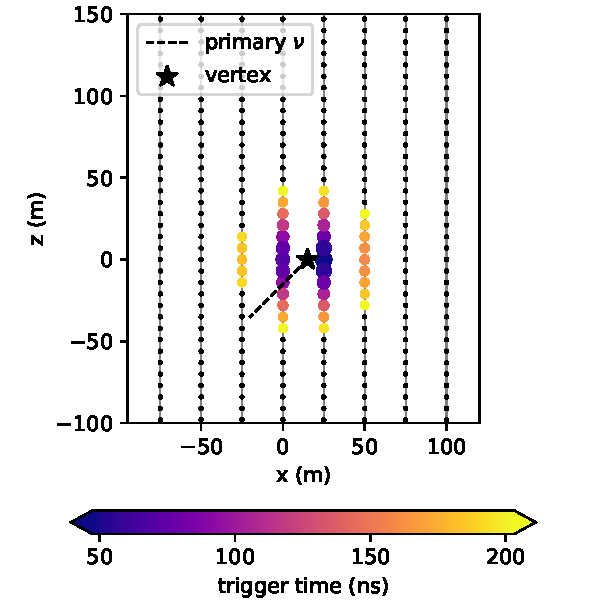
\includegraphics[width=0.49\textwidth]{figures/icecube/eventviews/idealized_cascade_view.pdf}
    \hfill
    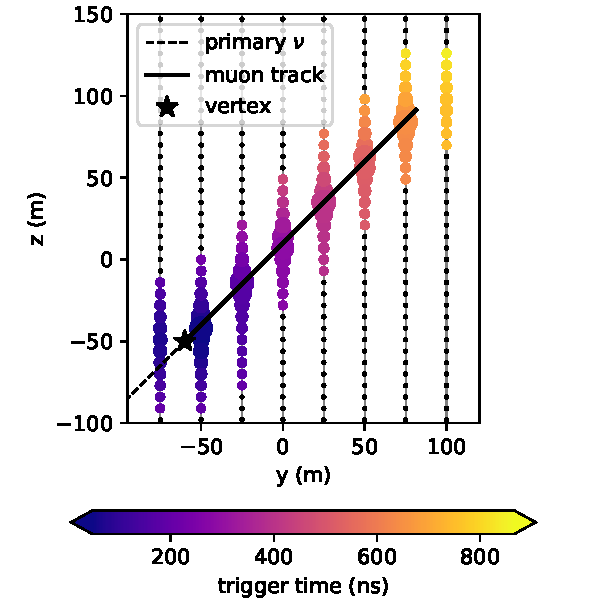
\includegraphics[width=0.49\textwidth]{figures/icecube/eventviews/idealized_track_view.pdf}
    \caption{An idealized cascade event (left) and starting track event (right) seen from the side. Each DOM that has received light is highlighted with a colored bubble, where the size is proportional the total charge seen by the DOM and the color indicates the time of the hits relative to the time at which the neutrino interaction happened.}
    \label{fig:idealized_signatures}
\end{figure}

% \begin{marginfigure}
%     \centering
%     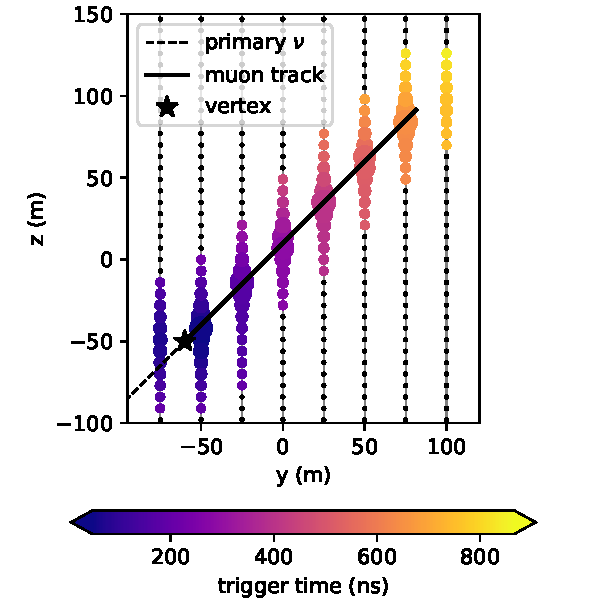
\includegraphics[width=\textwidth]{figures/icecube/eventviews/idealized_track_view.pdf}
%     \caption{An idealized \numucc-event seen from the side. Light is emitted uniformly from the interaction vertex as well as the endpoint of the track, and follows the Cherenkov cone along the track.}
%     \label{fig:idealized_track}
% \end{marginfigure}
% \begin{marginfigure}
%     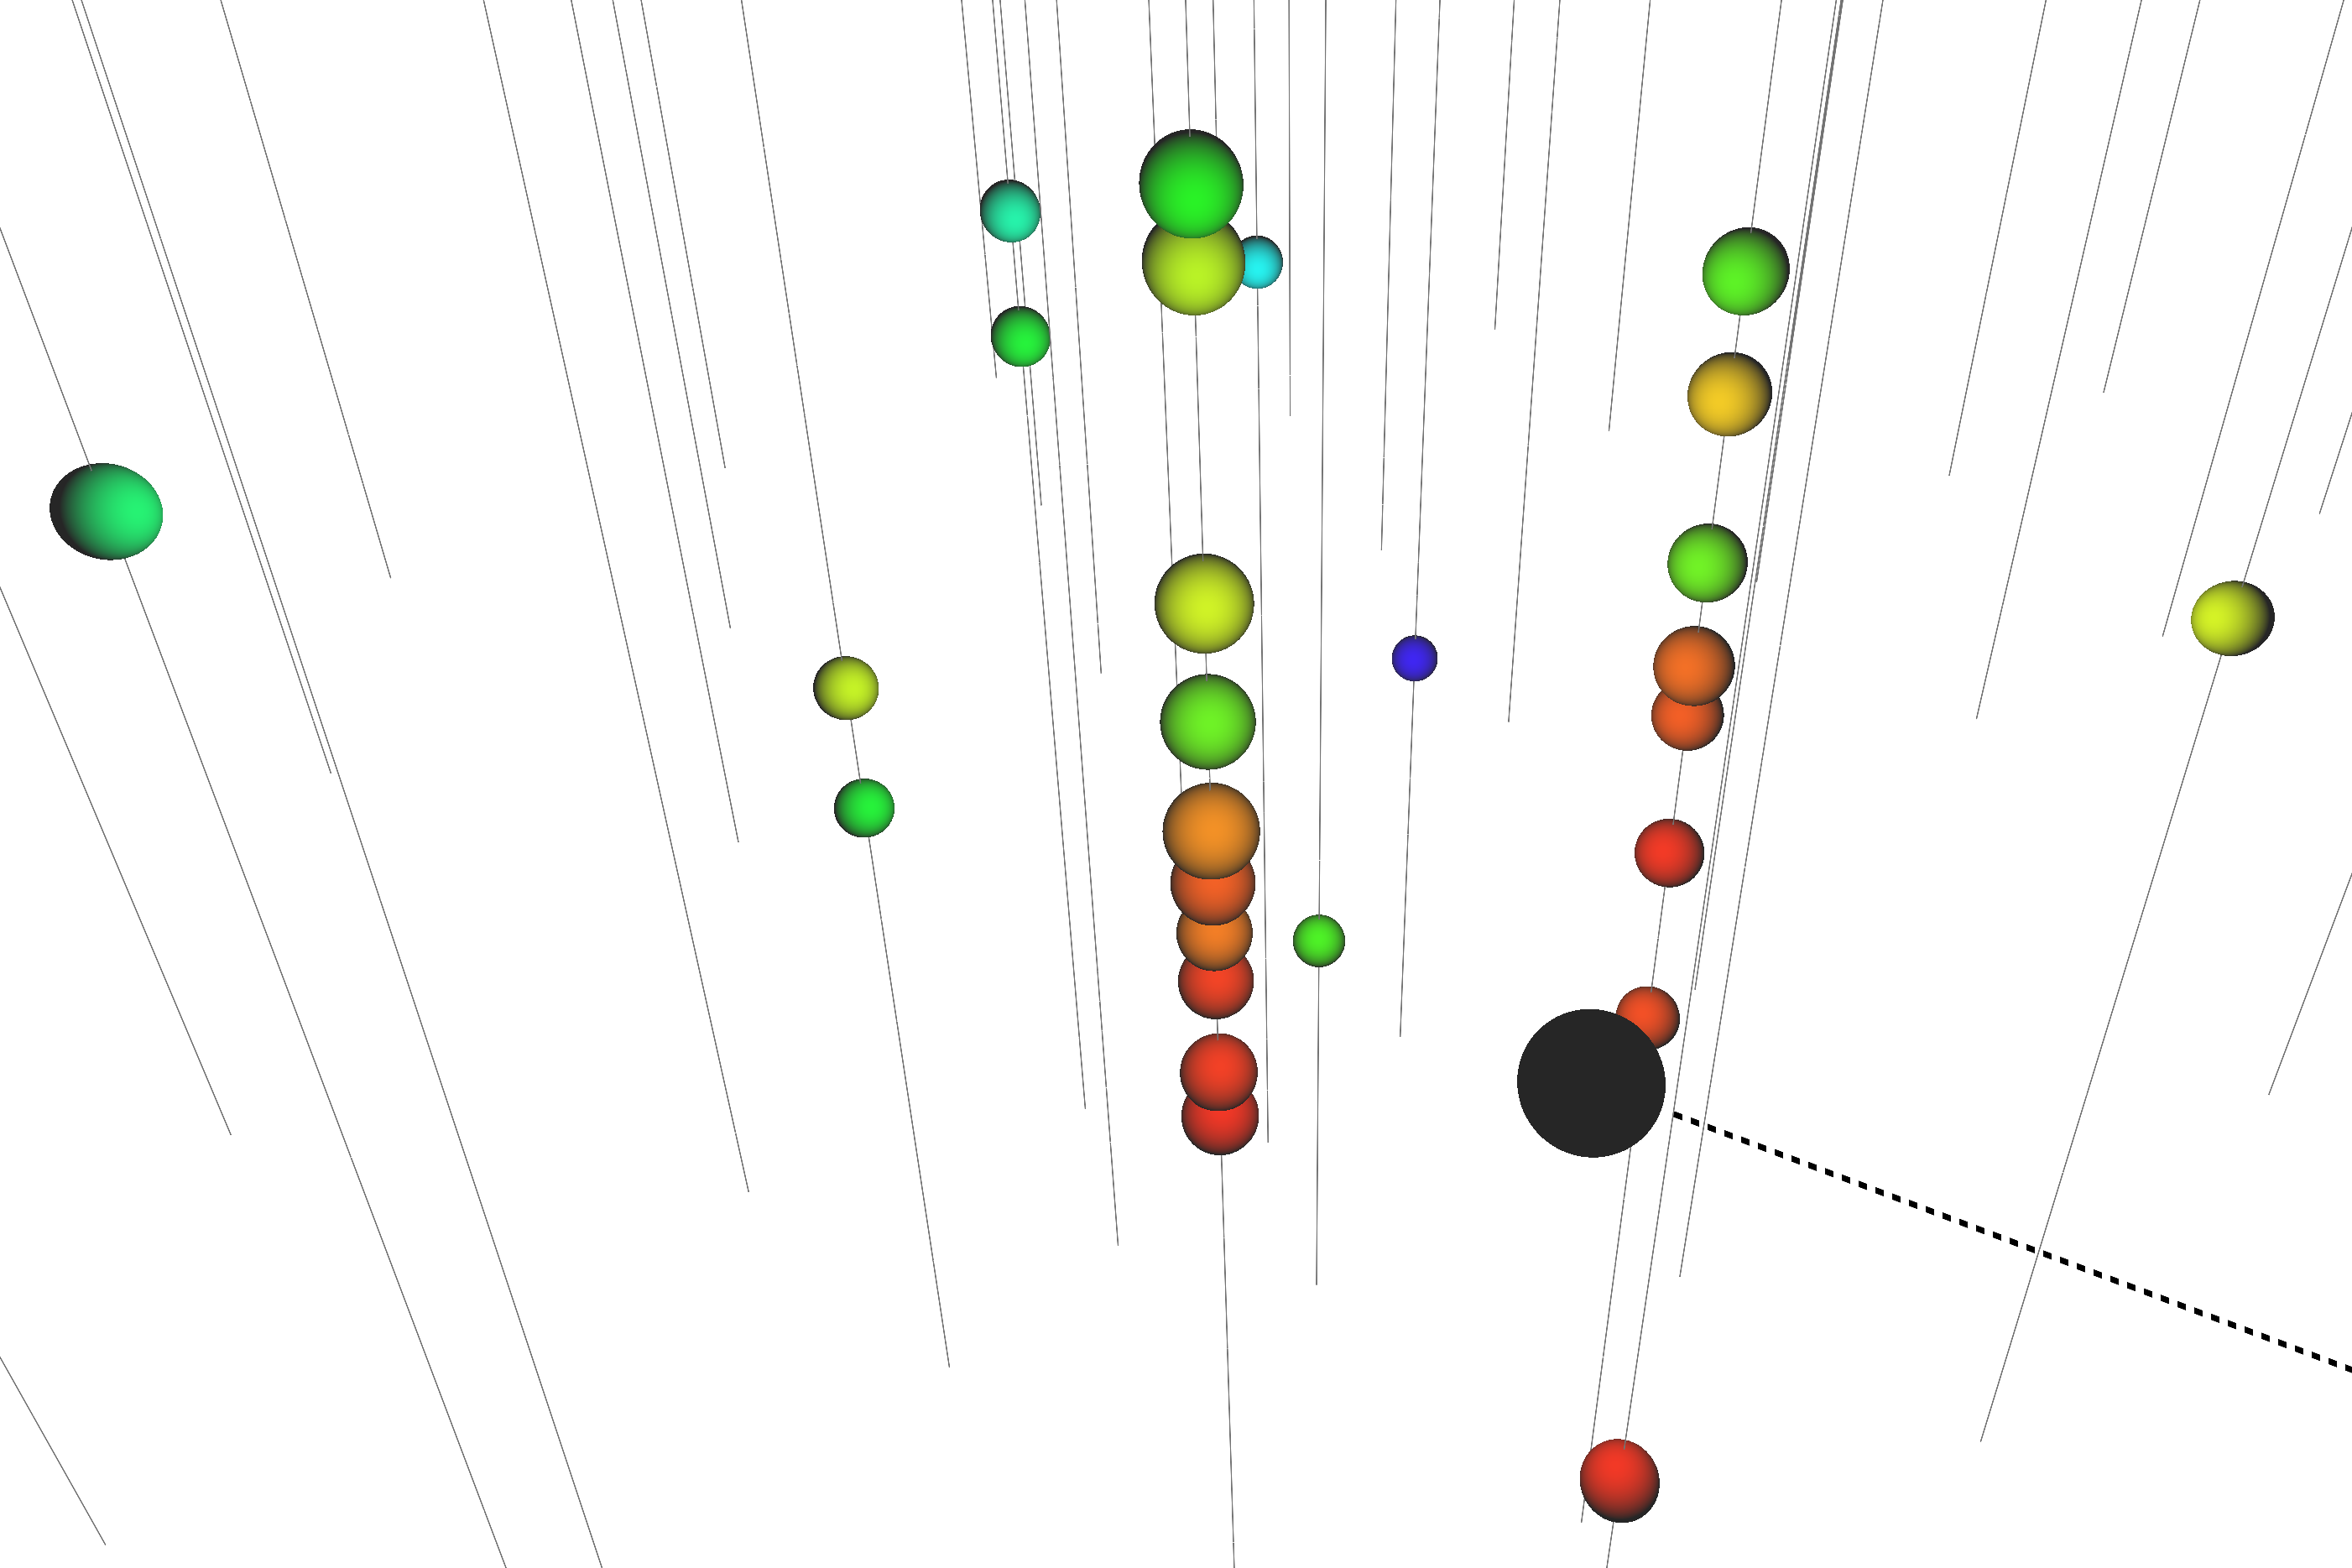
\includegraphics[width=\textwidth]{figures/icecube/eventviews/NuECC_with_neutrino_2_crop.png}
%     \caption{A simulated low energy $\nu_e$-CC neutrino interaction with an energy of 25 GeV inside the DeepCore sub-volume. The true neutrino direction is shown as the black dashed line, and the vertex as the black, round marker.}
%     \label{fig:emcasc-view}
% \end{marginfigure}
% \subsection{Tracks}
For muon-neutrinos, a muon is produced in the CC interaction which can then travel a significant distance through the ice beyond the extent of the initial hadronic shower, creating a track-like signature that sticks out of the cascade.
An idealized version of such an event is shown in the right panel of figure~\ref{fig:idealized_signatures}.

%The signal that such an interaction at an energy of 25~GeV produces in the DeepCore volume is shown in figure~\ref{fig:lowen-track-view}.
% \begin{marginfigure}
%     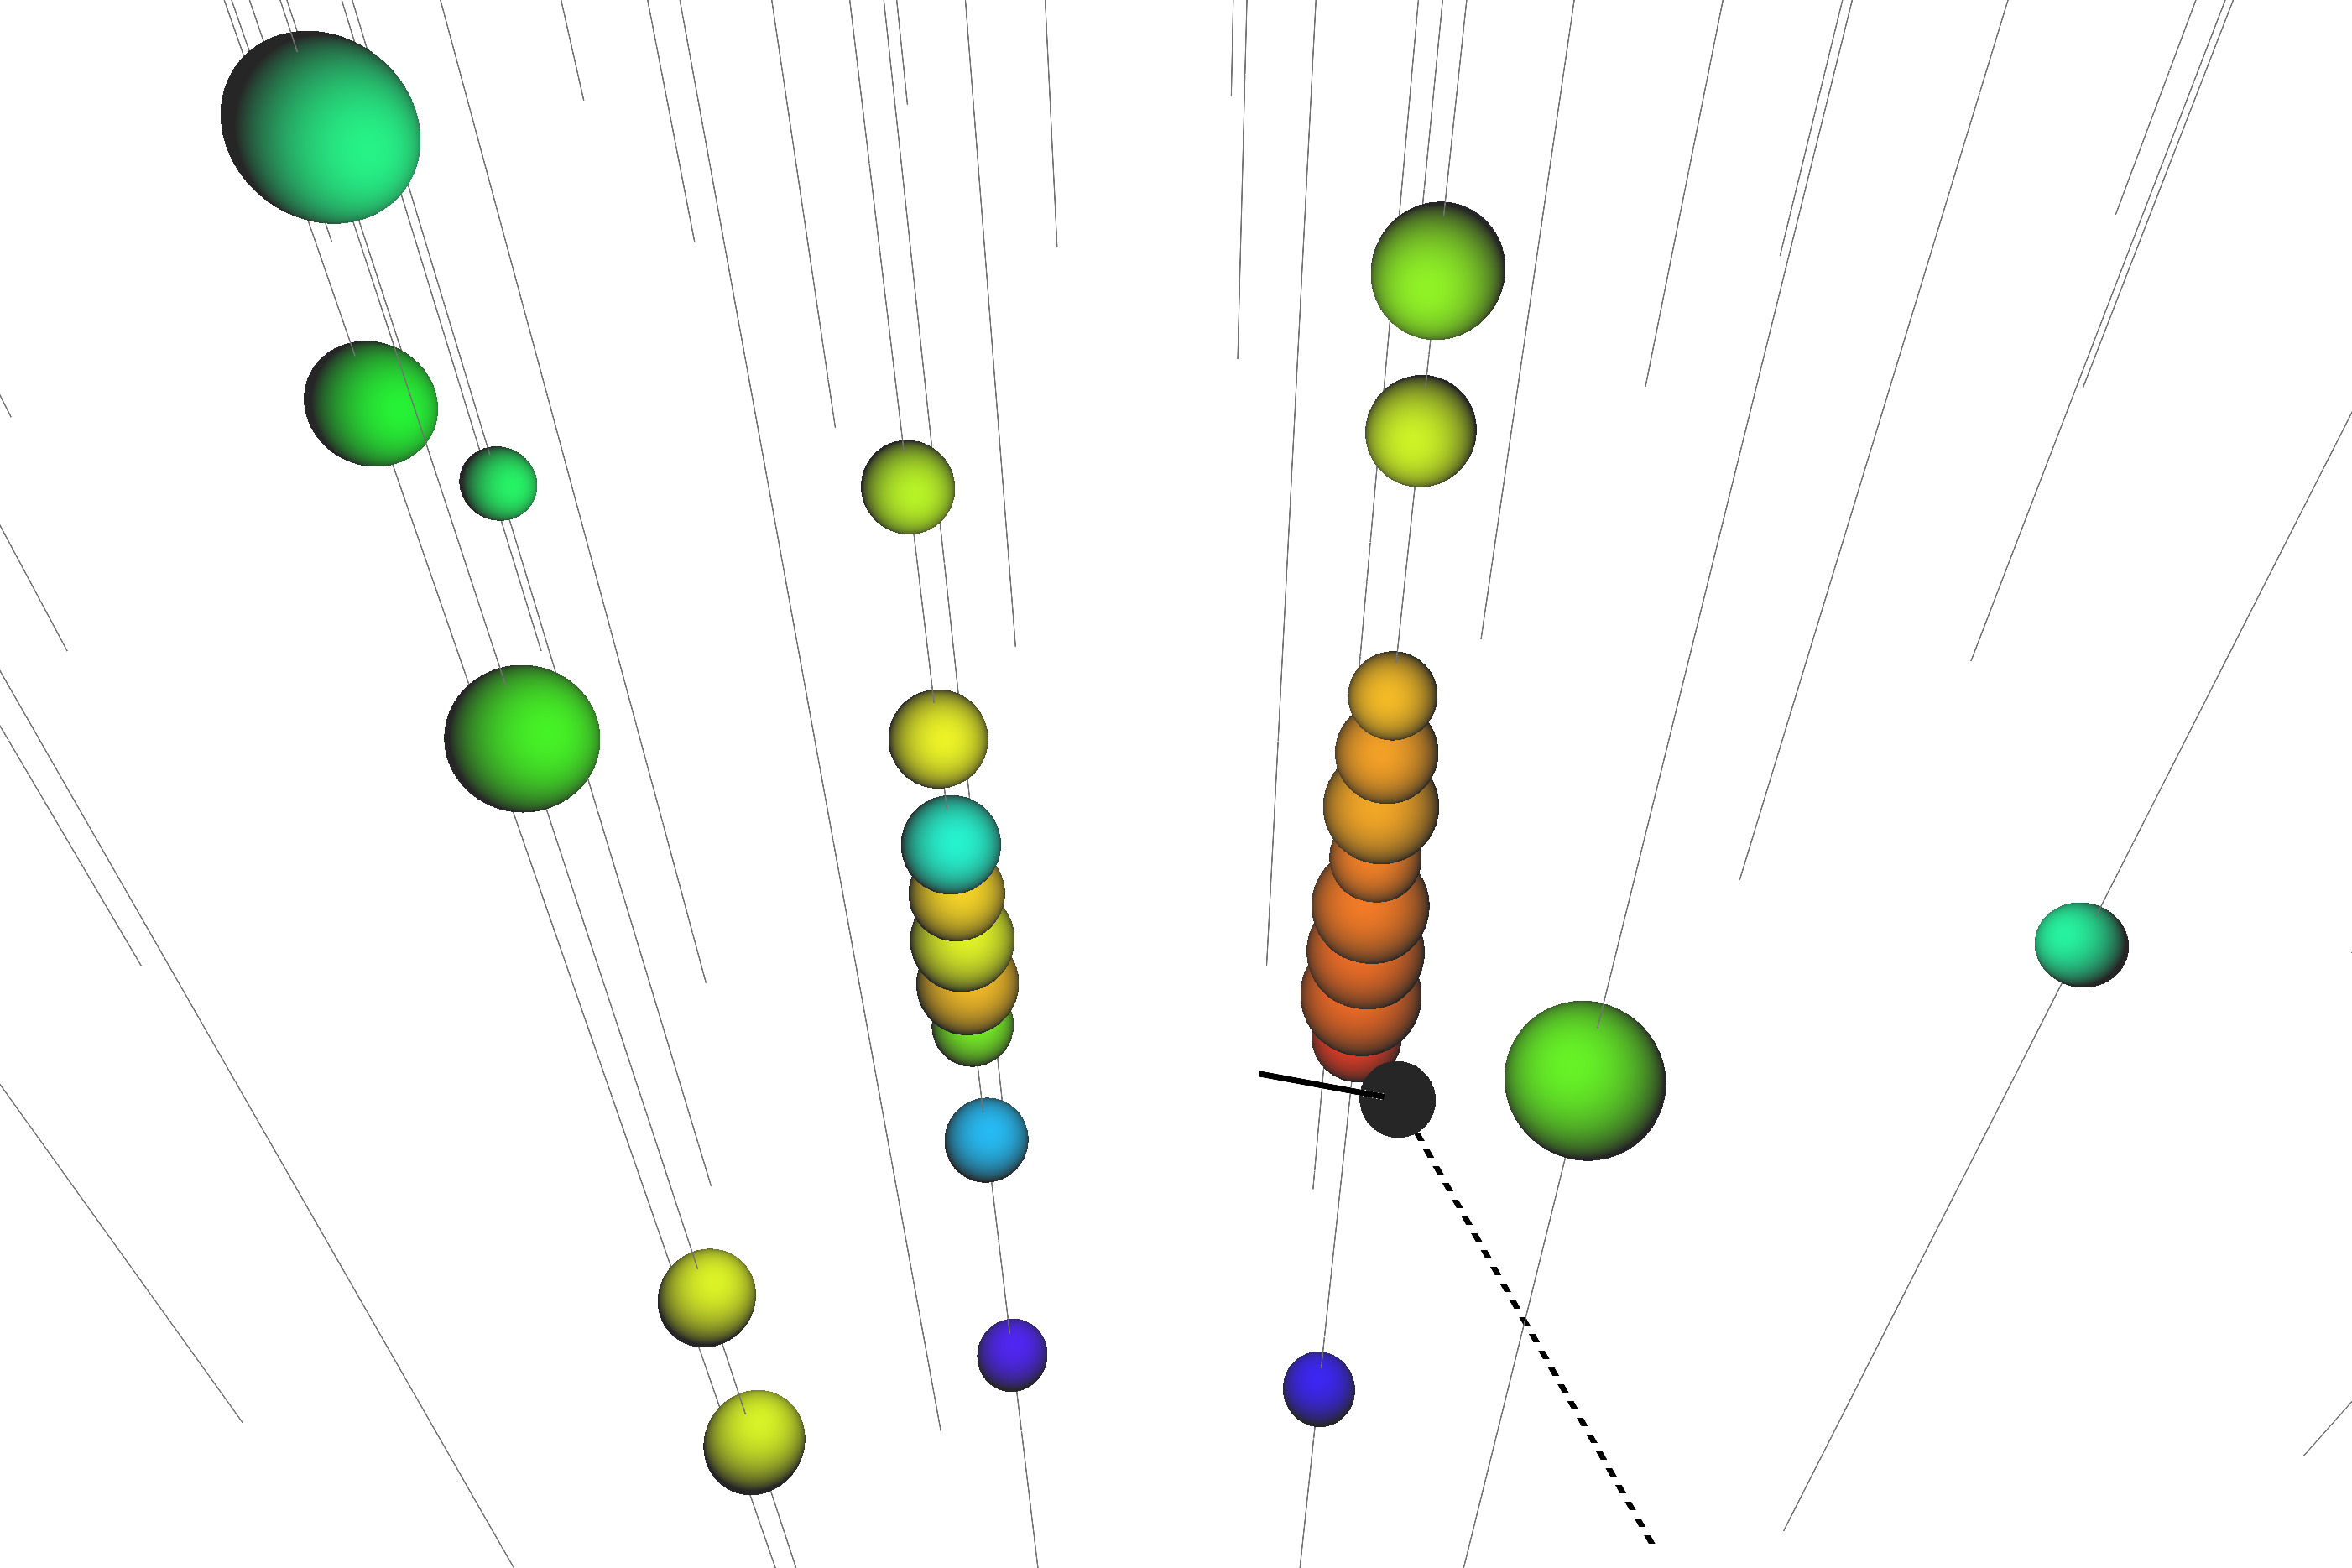
\includegraphics[width=\textwidth]{figures/icecube/eventviews/NuMuCC_with_neutrino_2_shorter_cmap_range_crop.png}
%     \caption{A simulated low energy \numucc neutrino interaction with an energy of 25~GeV inside the DeepCore sub-volume, with an outgoing 8 GeV $\mu^-$ indicated with the black, solid line (track).}
%     \label{fig:lowen-track-view}
% \end{marginfigure}
Charged-current interactions of tau-neutrinos produce a tauon that decays after a short distance, creating a second EM or hadronic shower at the point of its decay.
At TeV-scale energies, the distance covered by the tauon before its decay can be large enough to make the separation between the two showers resolvable, creating a \emph{double-bang} signature consisting of two cascades.
At energies below 100~GeV that are more relevant to this work, however, the two cascades are too close together to be cleanly separable and they are effectively approximated as a single cascade as well.
About 17\% of tauons produce a muon upon decay, creating a track-like signature as well\cite{pdg}.

A summary of the secondary particles and corresponding signatures for each type of neutrino interaction is given in \reftab{interaction-signatures}.
% \begin{marginfigure}
%     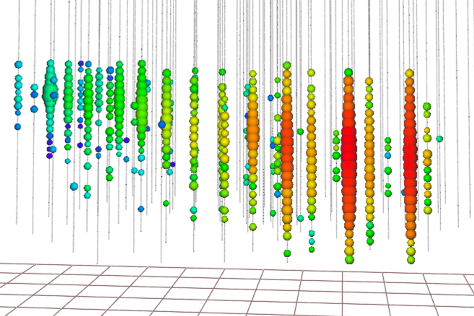
\includegraphics[width=\textwidth]{figures/icecube/eventviews/numucc_TeV_crop.png}
%     \caption{A high energy event (IceCube-170922A) with estimated energy of about 290 TeV. \cite{IceCube:2018dnn}}
%     \label{fig:txs-event}
% \end{marginfigure}

\tikzstyle{emcasc}=[shade,left color=blue!50,right color=blue!20, draw=blue]
\tikzstyle{hadcasc}=[shade,left color=red!50,right color=red!20, draw=red]
\tikzstyle{muon}=[draw=ProcessBlue, thick]
\tikzstyle{nu}=[densely dotted]
\tikzstyle{tau}=[draw=red]

\newcommand{\drawnuecc}{
    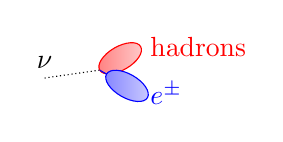
\begin{tikzpicture}
        \node (vertex) at (0, 0) {};
        \draw (-0.7, -0.1) node [anchor=south] {$\nu$} [nu] -- (vertex.center);
        \draw (vertex.center) +(0:0.3)[hadcasc,rotate=30] ellipse (0.3 and 0.15);
        \node [anchor=west,red] at (30:0.6) {hadrons};
        \draw (vertex.center) -- +(-30:0.1) +(0:0.4) [emcasc,rotate=-30] ellipse (0.3 and 0.15);
        \node [anchor=west,blue] at (-30:0.6) {$e^\pm$};
    \end{tikzpicture}
}

\newcommand{\drawnumucc}{
    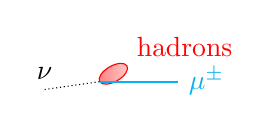
\begin{tikzpicture}
        \node (vertex) at (0, 0) {};
        \draw (-0.7, -0.1) node [anchor=south] {$\nu$} [nu] -- (vertex.center);
        \draw (vertex.center) +(0:0.2)[hadcasc,rotate=30] ellipse (0.2 and 0.1);
        \node [anchor=south west,red] at (30:0.4) {hadrons};
        \draw (vertex.center)[muon] -- +(0:1.0) node [anchor=west,ProcessBlue] {$\mu^\pm$};
    \end{tikzpicture}
}

\newcommand{\drawnutaucc}{
    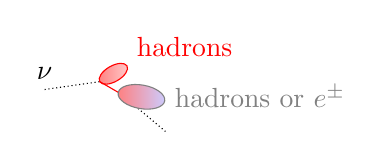
\begin{tikzpicture}
        \node (vertex) at (0, 0) {};
        \draw (-0.7, -0.1) node [anchor=south] {$\nu$} [nu] -- (vertex.center);
        \draw (vertex.center) +(0:0.2)[hadcasc,rotate=30] ellipse (0.2 and 0.1);
        \node [anchor=south west,red] at (30:0.4) {hadrons};
        \draw (vertex.center)[tau] -- +(-30:0.3) node (taudecay) {};
        \draw (taudecay.center) [nu] -- +(-40:0.75);
        \draw (taudecay.center) ++(10:0.3) [shade,left color=red!50,right color=blue!20, draw=gray,rotate=-10] ellipse (0.3 and 0.15) +(10:0.3) node [anchor=west,gray] {hadrons or $e^\pm$};
    \end{tikzpicture}
}

\newcommand{\drawnutauccmu}{
    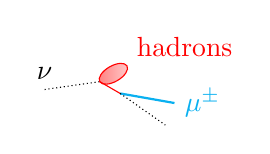
\begin{tikzpicture}
        \node (vertex) at (0, 0) {};
        \draw (-0.7, -0.1) node [anchor=south] {$\nu$} [nu] -- (vertex.center);
        \draw (vertex.center) +(0:0.2)[hadcasc,rotate=30] ellipse (0.2 and 0.1);
        \node [anchor=south west,red] at (30:0.4) {hadrons};
        \draw (vertex.center)[tau] -- +(-30:0.3);
        \draw (vertex.center) ++(-30:0.3)[muon] -- +(-10:0.7) node [anchor=west,ProcessBlue] {$\mu^\pm$};
        \draw (vertex.center) ++(-30:0.3)[nu] -- +(-35:0.7);
    \end{tikzpicture}
}

\newcommand{\drawnunc}{
    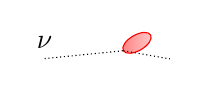
\begin{tikzpicture}
        \node (vertex) at (0, 0) {};
        \draw (-1, -0.1) node [anchor=south] {$\nu$}[nu] -- (vertex.center);
        \draw (vertex.center) +(0:0.2)[hadcasc,rotate=30] ellipse (0.2 and 0.1);
        \draw (vertex.center)[nu] -- +(-10:0.6);
    \end{tikzpicture}
}

\begin{table}
    \centering
    \begin{tabular}{p{0.1 \linewidth}cc}
         interaction & secondary particles & signature \\
         \toprule
         $\nu_e$ CC &  \drawnuecc &  cascade\\
         \midrule
         $\nu_\mu$ CC &  \drawnumucc &  cascade + track\\
         \midrule
         $\nu_\tau$ CC (83\%~BR) &  \drawnutaucc &  cascade\\
         $\nu_\tau$ CC (17\%~BR) &  \drawnutauccmu &  cascade + track\\
         \midrule
         $\nu$ NC &  \drawnunc &  cascade\\
    \end{tabular}
    \caption{Secondary particles and signatures produced by each type of neutrino interaction.}
    \label{tab:interaction-signatures}
\end{table}

\subsection{Atmospheric muons}
Atmospheric muons are a significant background for oscillation measurements in DeepCore.
Not only do they make up the majority of events that pass the initial DeepCore filter, but they also produce a track-like signature in the detector that is challenging to separate from that of a charged-current muon neutrino interaction.
For this reason, most of the data filtering steps described in \refsec{offline-filter} are devoted to rejecting atmospheric muons while keeping as many muon neutrinos in the sample as possible.
At energies below 100~GeV, the dominant energy loss for muons is ionization, which creates a continuous energy loss that can pass through the entirety of the instrumented volume of IceCube.
As energies increase above 100~GeV, radiative energy losses become more relevant that create a series of stochastically distributed cascades along the muon's trajectory.
The fraction of total energy loss that is concentrated in these cascades is referred to as \emph{stochasticity}.
Atmospheric muons also often arrive in bundles originating from a single interaction of cosmic rays with the upper atmosphere.
Within such a bundle, stochastic energy losses of individual muons may average out over its trajectory, such that the bundle as a whole can be approximated as a single long track with a relatively low stochasticity.


% \subsection{Systematic uncertainties not included in the measurement}
\label{sec:other-uncertainties}

Several other potential sources of systematic uncertainties were investigated during the development of the analysis presented in this work whose impact was found to be negligible.


\subsubsection{Other oscillation parameters}
\label{sec:other-oscillation-syst}

The impact of other oscillation parameters besides $\theta_{23}$ and $\Delta m^2_{13}$ on the observed signal was assessed within the bounds set by other experiments and was found to be negligible. One exception is the CP-violating phase $\delta_{\mathrm{CP}}$, which had the potential to cause a small bias in the analysis as described in the assessment of parameter impact in \refch{measurement-three-flavor}. The analyses presented in this work only test the hypothesis under which $\delta_{\mathrm{CP}}=0$ for simplicity and to produce a result that is directly comparable to that of other experiments.

\subsubsection{Depth-dependent ice properties}
\label{sec:depth-dependent-ice-properties}

In the parametrization of the uncertainties of the detector properties described in \refsec{detector-unc}, variations of the scattering and absorption coefficients are only described by global, depth-independent scaling factors.
In principle, the error on the properties of the ice could also change as a function of depth.
For instance, one would expect that the uncertainty on the ice absorption is larger in regions with increased dust deposition, because the dust will absorb the LED light that is used to calibrate the ice model.
Of particular interest for the analysis presented in this work are variations of the ice properties at length scales of the DeepCore fiducial volume located within DeepCore.
Variations at much longer scales would be indistinguishable from uniform variations given the size of the event signatures observed below 100~GeV, while variations at much shorter scales are expected to average out.
To test how significantly such a variation would impact the final level histograms, two MC sets are produced in which the scattering and absorption coefficients vary following a sigmoid function function centered in DeepCore with an amplitude of $\pm 2\%$ in opposing directions as shown in \reffig{step-function-ice-model}.
\begin{figure}
    \centering
    \missingfigure[figwidth=0.8\linewidth]{Show step function variations, see  \href{https://drive.google.com/file/d/1TV0r1VzRbRPxlQeeCuq8DaZzeQloJZ_J/view}{presentation on lowen call}.}
    \caption{Perturbation of the scattering and absorption coefficients with respect to the nominal ice model applied in additional MC sets.}
    \label{fig:step-function-ice-model}
\end{figure}
The size of this variation corresponds approximately a $1\sigma$-allowed variation according to flasher calibration data. Then, for every bin in the final analysis histogram, a linear regression is fit to the bin counts of the nominal MC set and the two variations assuming that they correspond to $\pm 2\%$ variations of a parameter.
The resulting slopes were found to be indistinguishable from pure statistical variation and it was concluded that the impact of such a hypothetical new systematic uncertainty would be insignificant.\todo{This was only done for the high-stats sample: redo for verification sample?}

%In previous oscillation studies using track-like events in the TeV energy range \sidecite{MEOWS}, this effect was found to be non-negligible. To model depth-dependent uncertainties of the ice properties, a method was developed in which the depth-dependence of the scale factor for scattering and absorption coefficients is decomposed into Fourier-modes, and the impact of each mode on the final analysis histogram can be calculated\sidecite{snowstorm}. In the analysis presented in \cite{MEOWS}, the impact of high-frequency Fourier modes was found to be negligible and therefore the uncertainties of the bulk ice was modeled using the lowest fourth modes.

\subsubsection{Atmospheric density}
\todo[inline]{Describe test of atmospheric density impact (or get feedback if that is even necessary}

\subsubsection{$K/\pi$-air interactions}
\todo[inline]{Describe this part, although it might also be just too much.}

% \section{Data Processing}
\label{sec:data-processing}

\subsection{Trigger}
As described in section \ref{sec:dom-daq}, the high-frequency ATWD waveform digitization in each DOM is triggered when it and its adjacent or next-to-adjacent neighbors on the same string record a voltages of at least 0.25 PE-equivalent within a $\pm$1~$\mu$s time window, which is referred to as the Hard Local Coincidence (HLC) condition. Data acquisition for DeepCore is triggered when this condition is fulfilled for at least three DOMs inside the DeepCore fiducial volume within a $\pm$2.5~$\mu$s window. If this condition is met, the waveforms for all DOMs that have observed voltages of at least 0.25~PE within a $\pm$10~$\mu$s time window centered around the trigger time are recorded. A DOM that is included in this readout but for which the HLC condition has not been met is said to fulfill the \emph{Soft Local Coincidence} (SLC) condition. The DeepCore trigger rate is less than 10~Hz and will trigger on \~70\% of $\nu_\mu$ events at 10~GeV and >90\% of $\nu_\mu$ events at 100~GeV\cite{DeepCore}.

\subsection{Online Filter}

Once the trigger condition is met, the recorded waveforms within the trigger window are converted into reconstructed pulses and are then passed into a set of \emph{online} filters (i.e. filters running on hardware at the Pole). These filters are each designed to select events that are relevant to different physics measurements that are performed within the IceCube collaboration. For the purposes of the analysis presented in this thesis, events are selected using the \emph{DeepCore filter}. This filter is designed to select events that start inside the DeepCore fiducial volume and to reject those that are consistent with muons entering the detector from the outside.
\begin{marginfigure}
    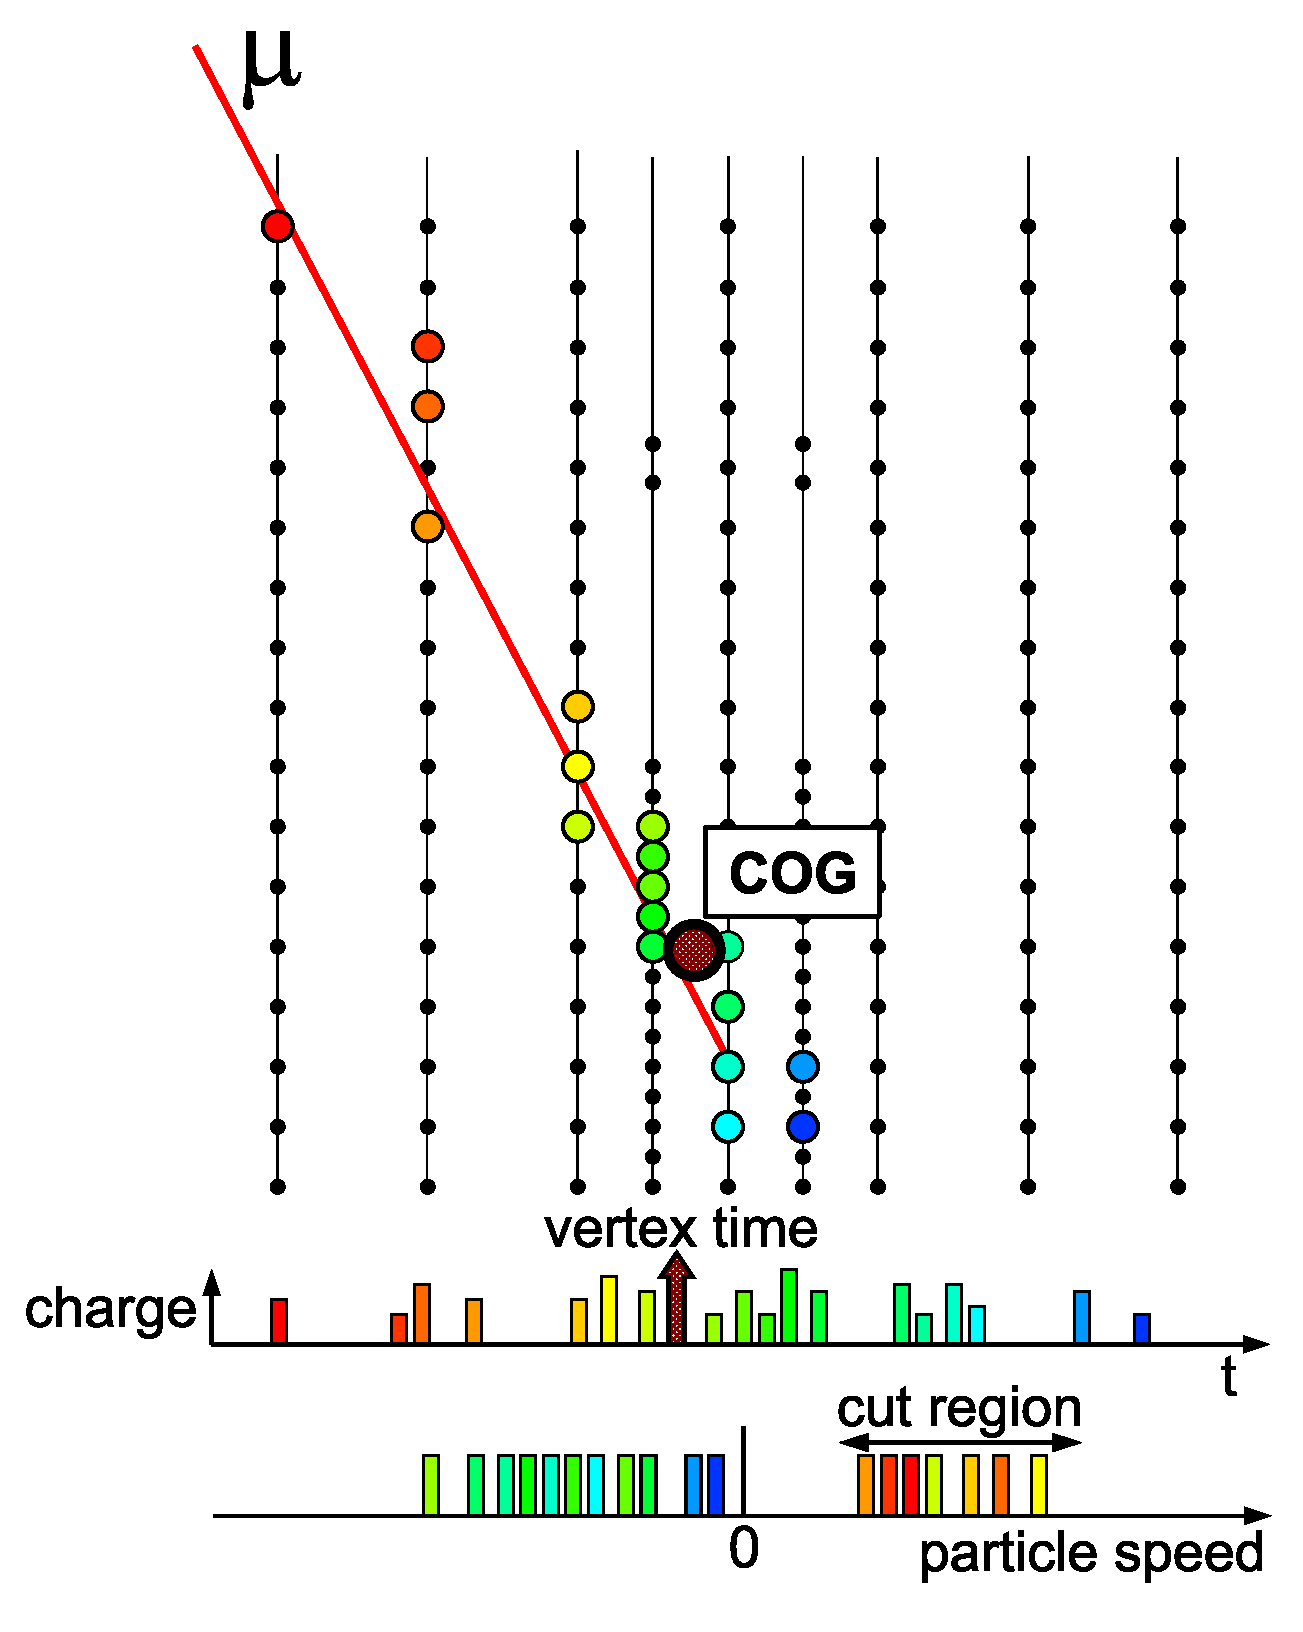
\includegraphics[width=\textwidth]{figures/icecube/eventviews/FilterDiagram.pdf}
    \caption{Example of an event that would be rejected by the online filter algorithm. DOMs that have observed light are highlighted in color depending on time from red (early hits) to blue (late hits). DOMs that have not observed any light are shown as black dots. Figure taken from \cite{DeepCore}.}
    \label{fig:online-filter-event}
\end{marginfigure}
The filter first applies a noise cleaning algorithm based on a coincidence condition between hits on different DOMs, where hits in DOMs for which the HLC condition was met are always kept. The cleaned hit series is split between those hits that fall within the DeepCore fiducial volume and those outside of it. The veto algorithm then calculates the COG in space and time of the hits inside the fiducial volume and then the velocity that a signal would have to travel from each hit occurring outside the fiducial volume to coincide with the COG. If this velocity is close to the speed of light (between $0.25\;\mathrm{ns/s}$ and $0.4\;\mathrm{ns/s}$) for at least one hit, the event is rejected because it is consistent with a muon traveling through the veto region and entering DeepCore. Figure~\ref{fig:online-filter-event} shows an example of an event that would be rejected by the online filter. Only events passing the trigger and filter condition are sent North via satellite for further \emph{offline} filtering.

\subsection{Offline Filter}

The offline filter is separated into subsequently applied \emph{levels}, referred to as L3, L4, and L5, where each level reduces the amount of background (atmospheric muons and noise) by approximately an order of magnitude while keeping most of the DeepCore starting events that are the target of the selection.

\subsubsection{Level 3}
At the lowest offline filter level, L3, cuts are applied to simple variables that remove the most easily identifiable background events while using only few computational resources. The variables aimed at cutting noise consist mostly of different DOM hit counts within hit series to which noise cleaning algorithms have been applied. The cuts aimed at removing muons consist of conditions on the number of hits in the veto region as well as conditions on the vertical position of the first HLC hit. The distribution for one of the variables used in the L3 filter is shown in figure~\ref{fig:l3-var-cleaned-full-time-length}. It is apparent from the distributions that there is a significant population of events in data with large values of the plotted variable that does not exist in simulation. These events are discarded, improving the agreement between data and simulation for events passing the L3 filter.
\begin{figure}
    \centering
    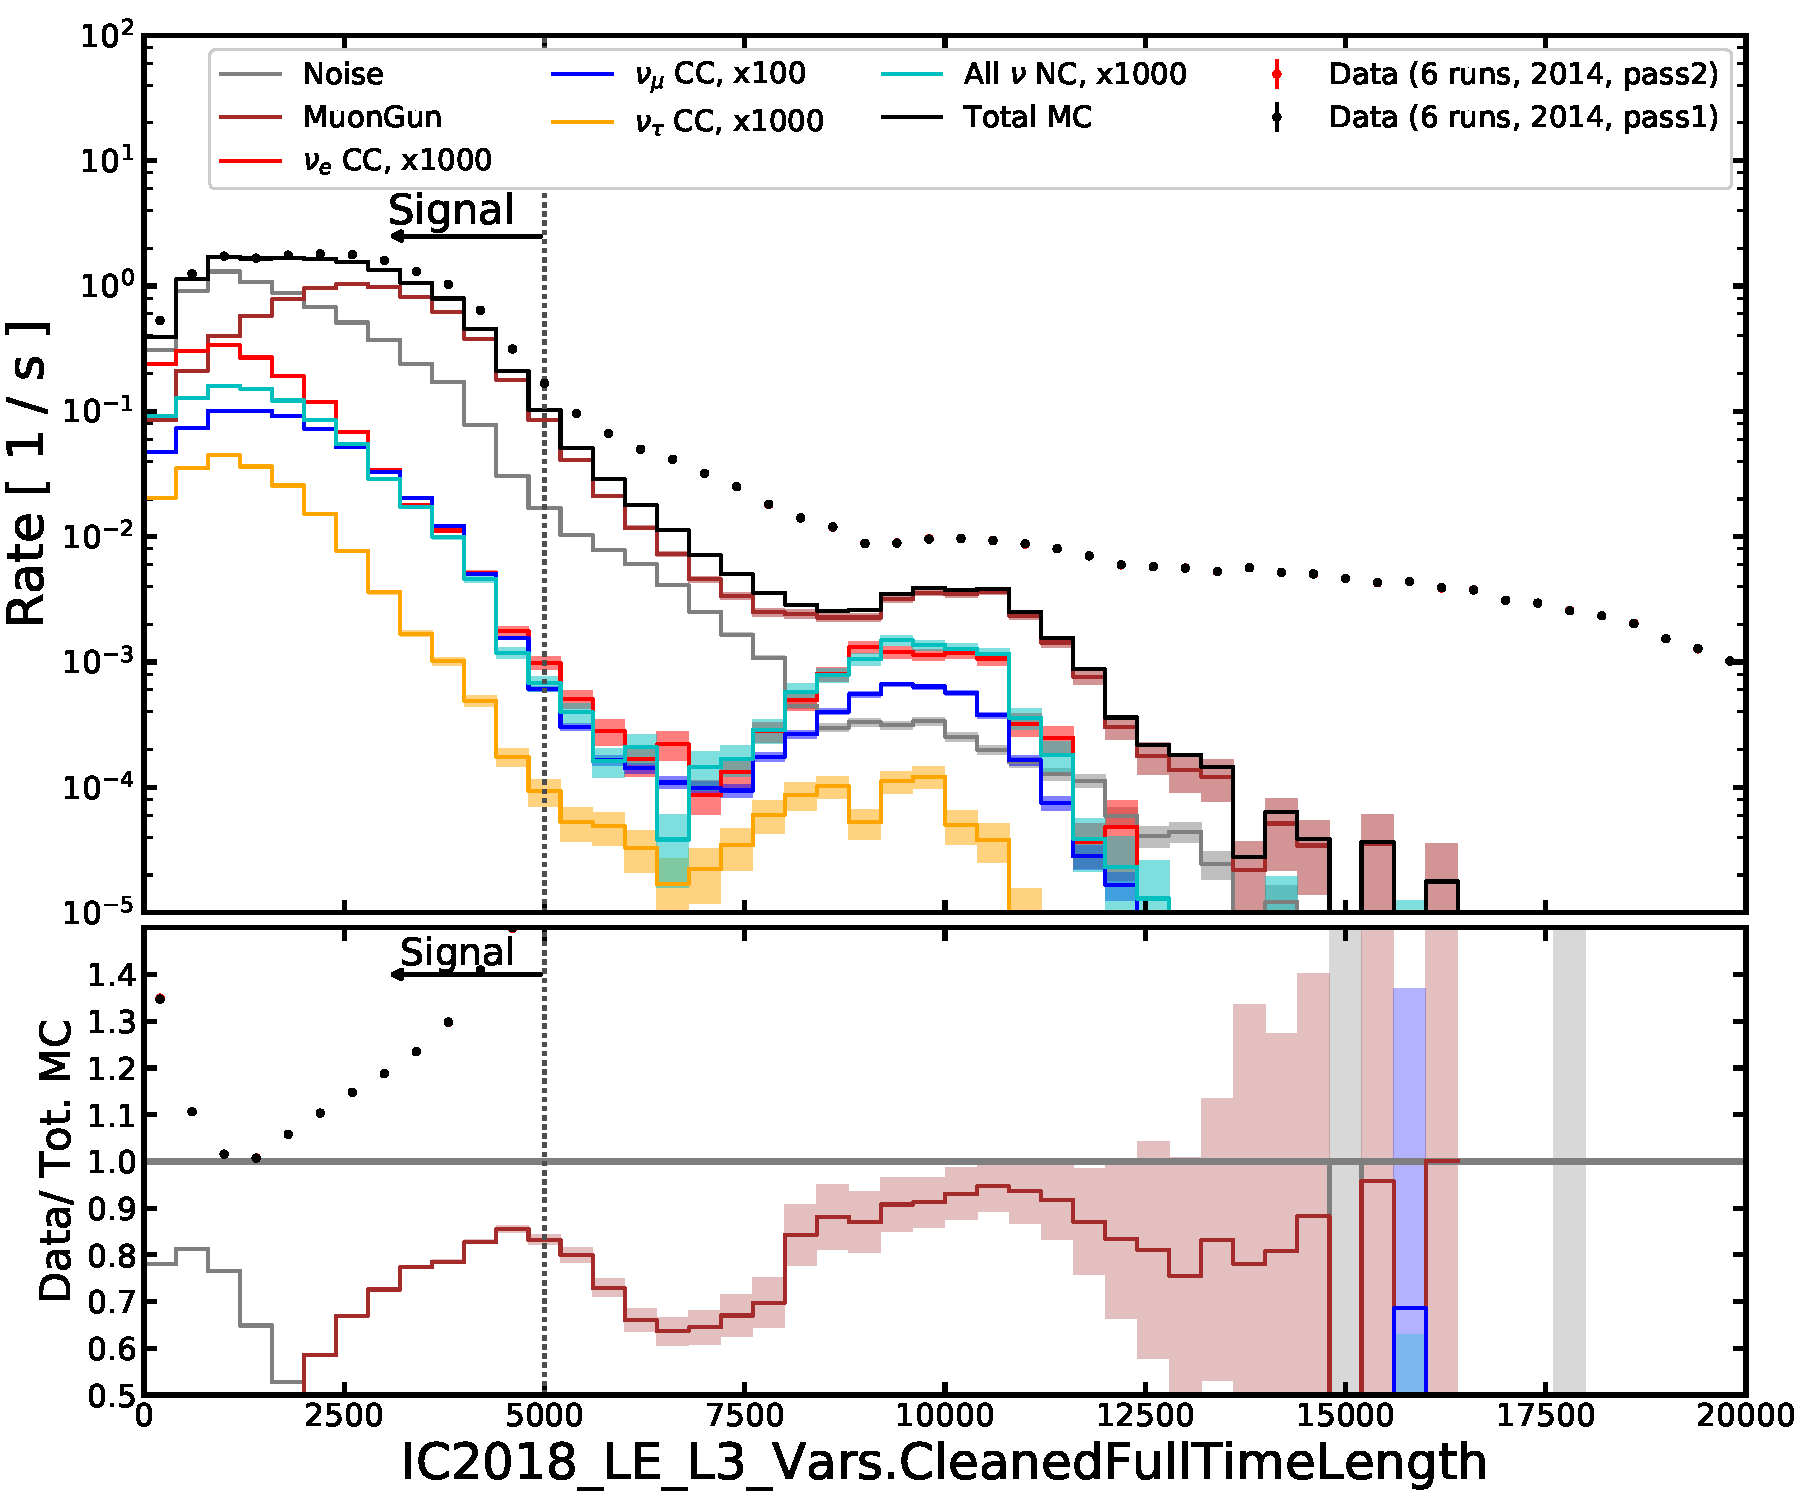
\includegraphics[width=7 cm]{figures/icecube/selection/IC2018_LE_L3_Vars_CleanedFullTimeLength.pdf}
    \caption{Distribution of one of the variables used in the L3 offline filter, the time between the last hit and the first hit after noise cleaning. Histograms show the distributions in simulated data separated by particle and interaction type, data points with error bars show the distribution of real data. The bottom panel shows the ratio between data and simulation. Events falling on the "signal" side of the histogram are passed to the next filter level.}
    \label{fig:l3-var-cleaned-full-time-length}
\end{figure}

\subsubsection{Level 4}
In the next level, L4, more advanced selections based on the output of Boosted Decision Trees (BDTs) are applied, with a separately trained BDT for noise and muon rejection, respectively. The output of each BDT is a probability score between zero (background-like) and one (signal-like).  The inputs into the BDT aimed at noise rejection consist of hit counts in cleaned hit series and variables that characterize the geometric and temporal spread of the observed hits, such as the full width half maximum (FWHM) of the hit times. The BDT is trained using simulated pure noise and neutrino events. Events are passing the L4 noise cut if the BDT score is above 0.7, which reduces the number of pure noise events by two orders of magnitude from 36.6~mHz to approximately 0.3~mHz. The BDT that is used to reject atmospheric muons also takes simple variables as its input that consist mostly of different veto hit counts and variables that characterize the distribution of z-coordinates of the observed hits as well as their radial distance with respect to the center of the DeepCore fiducial volume. In contrast to the noise BDT, however, the muon BDT is trained using real data and simulated neutrino events, with the goal of rejecting data events. This is possible because the data sample consists to 99\% of atmospheric muons at this stage of the event selection. Events are passing the L4 muon cut if the output score from the muon BDT is above 0.65, removing 94\% of all muon events while keeping 87\% of all neutrinos. The distributions of the output scores of both BDTs are shown in figure~\ref{fig:l4-bdt-output}.
\begin{figure*}
    \centering
    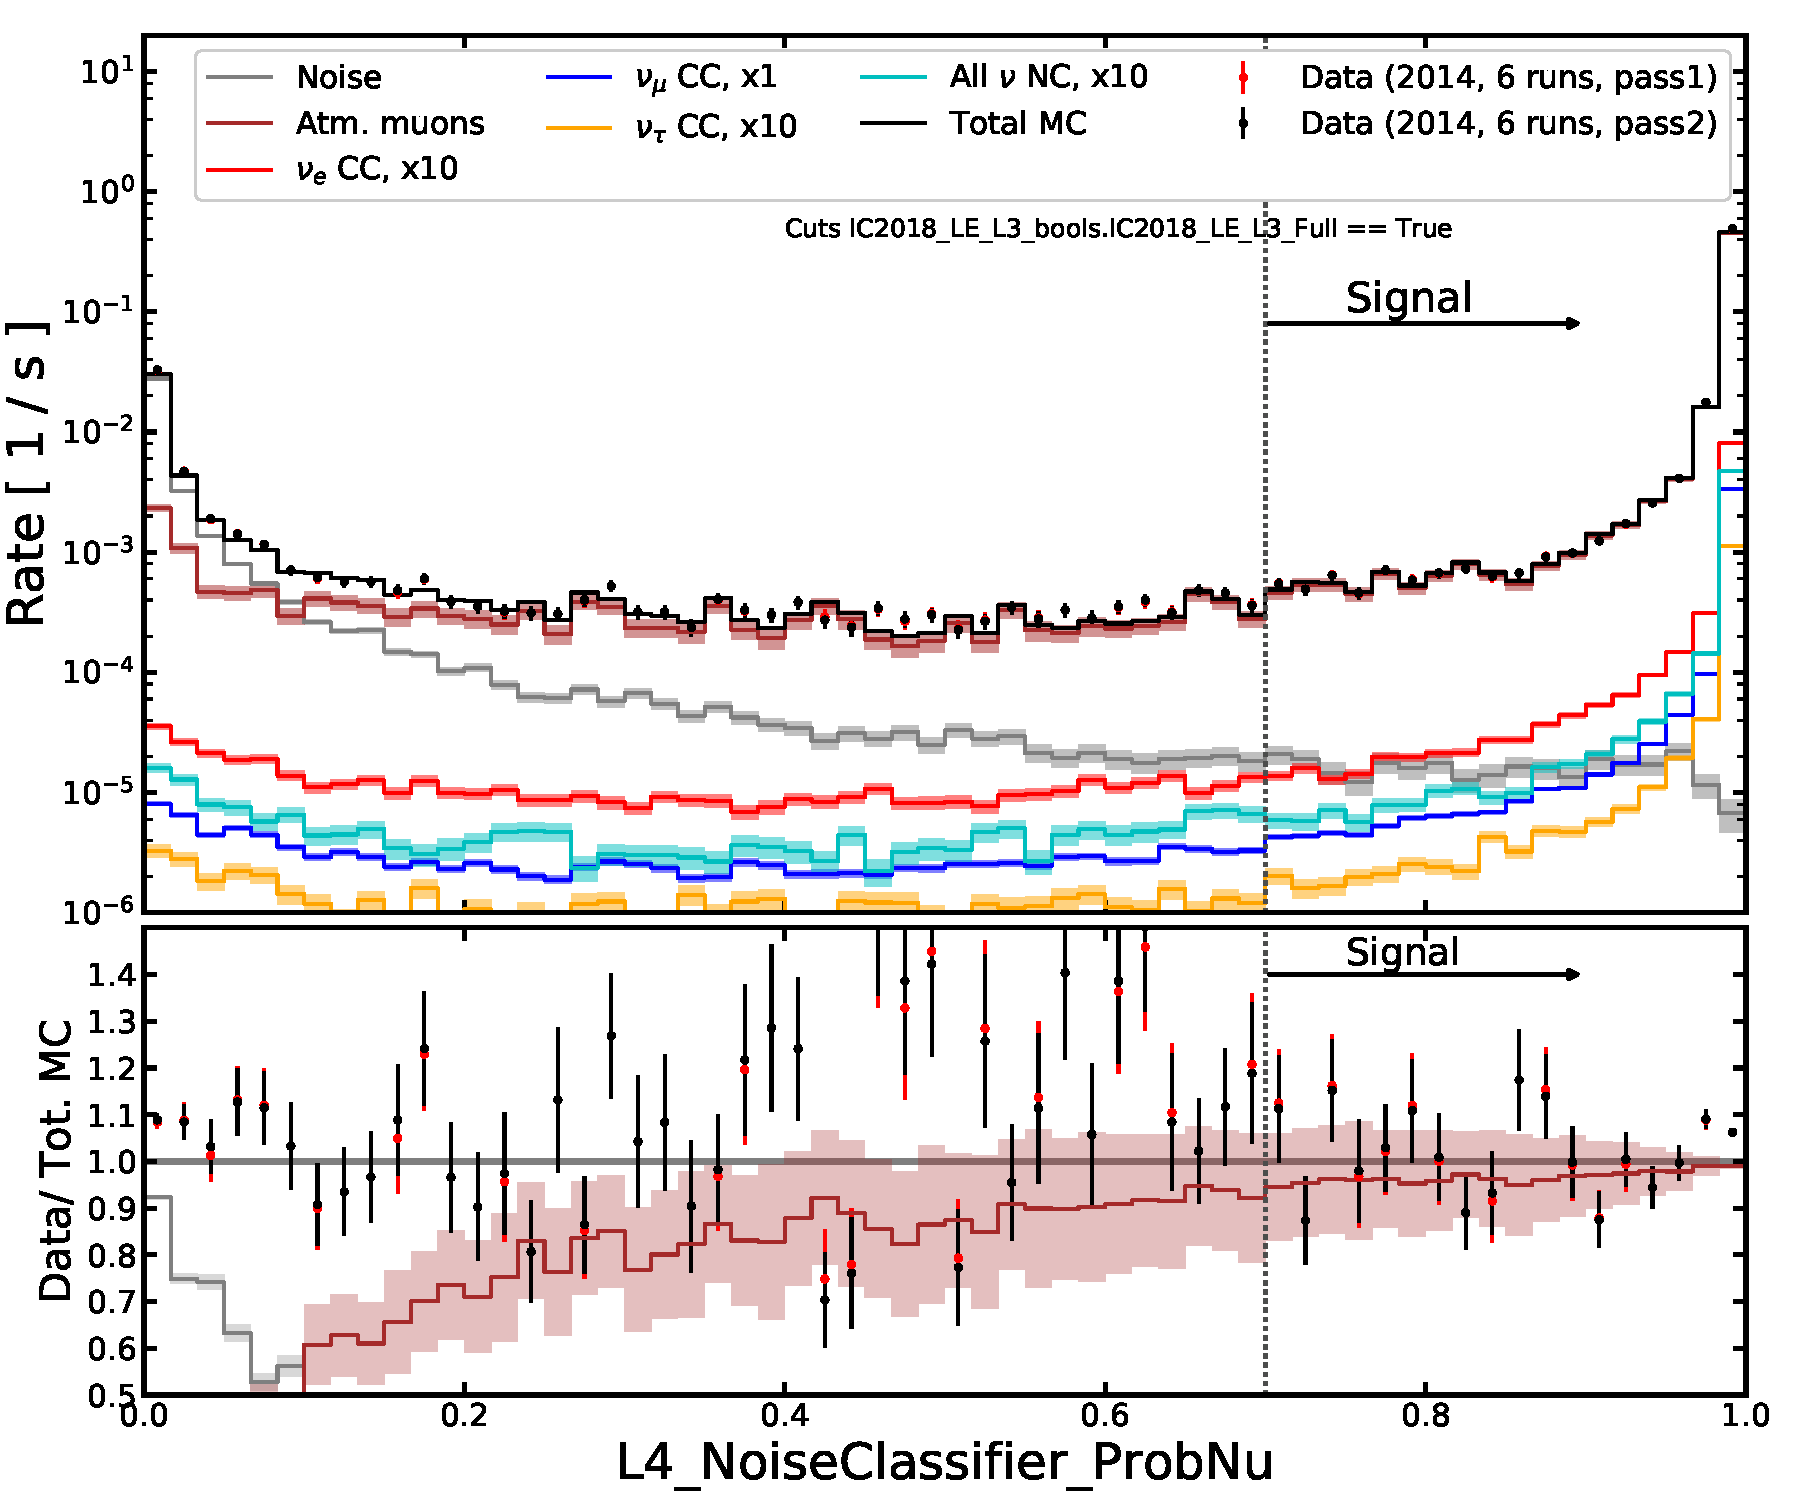
\includegraphics[width=7 cm]{figures/icecube/selection/L4_noiseBDT_L4_NoiseClassifier_ProbNu.pdf}
    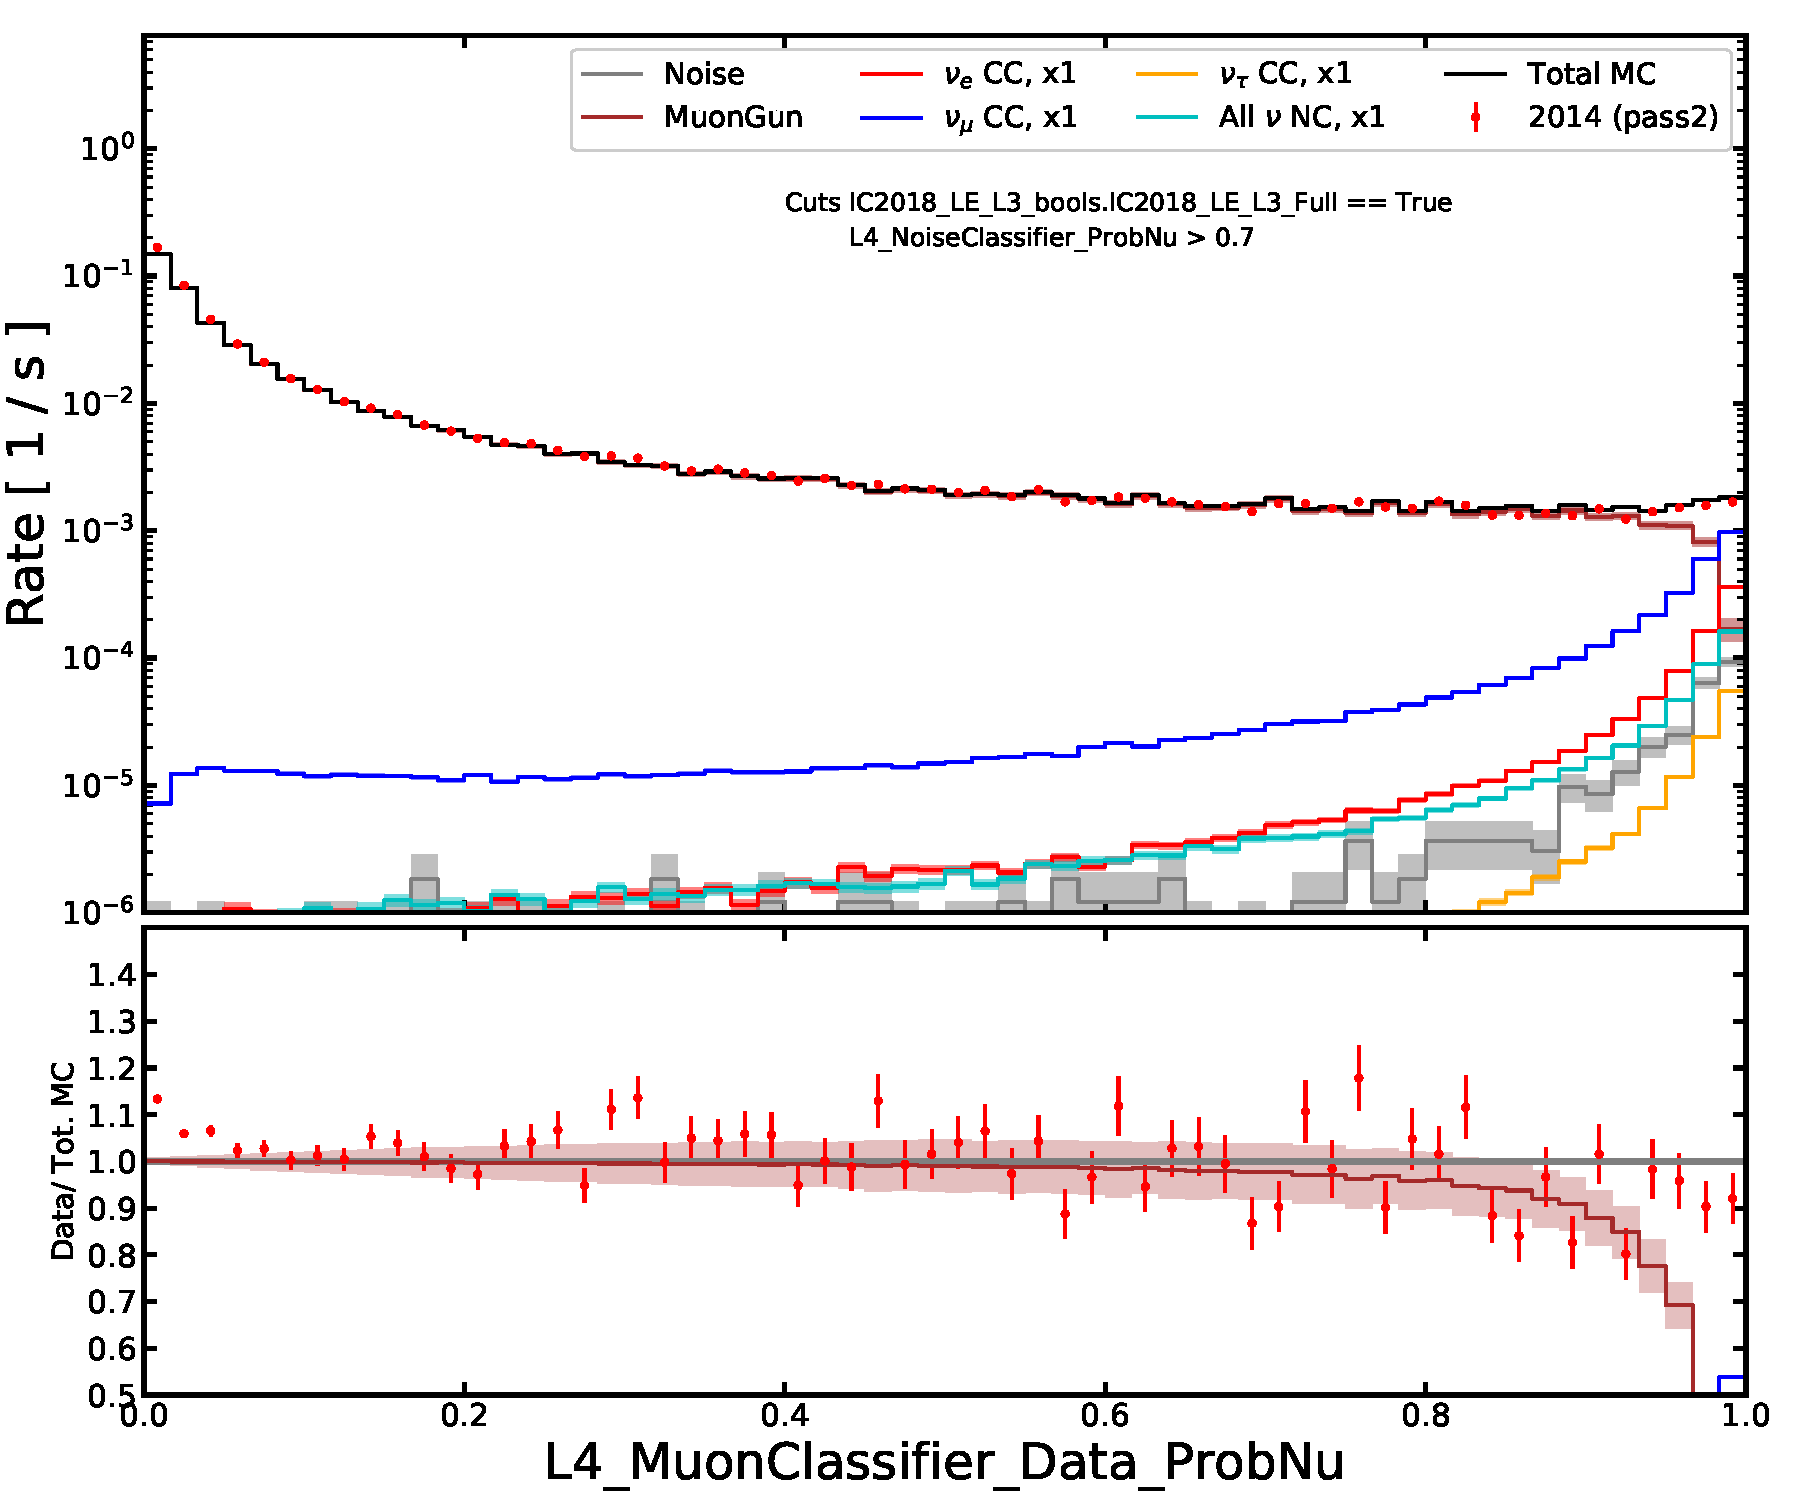
\includegraphics[width=7 cm]{figures/icecube/selection/L4_muon_L4_MuonClassifier_Data_ProbNu.pdf}
    \caption{Distribution scores for the noise (left) and muon (right) BDT. The distributions of the muon classifier are shown for events where the score of the noise BDT is greater than 0.7.}
    \label{fig:l4-bdt-output}
\end{figure*}

\subsubsection{Level 5}
The final offline filter level that is applied before the event reconstruction step is L5. This filter searches specifically for hits occurring in un-instrumented \emph{corridors} within the IceCube array through which an atmospheric muon can sneak into the DeepCore volume while evading previous veto cuts. In addition, events with more than seven hits in the outermost strings of the IceCube array or that have a down-going pattern of hits in the uppermost region of the detector are vetoed to remove events containing atmospheric muons entering the detector coincidentally with neutrinos. The distribution for one of the corridor variables and one of the muon rejection variables are shown in figure~\ref{fig:l5-vars}. Table~\ref{tab:l5_summary} shows the rates of each event type expected at each level of the selection up to L5 together with the efficiency of the filter at the final level.
\begin{figure*}
    \centering
    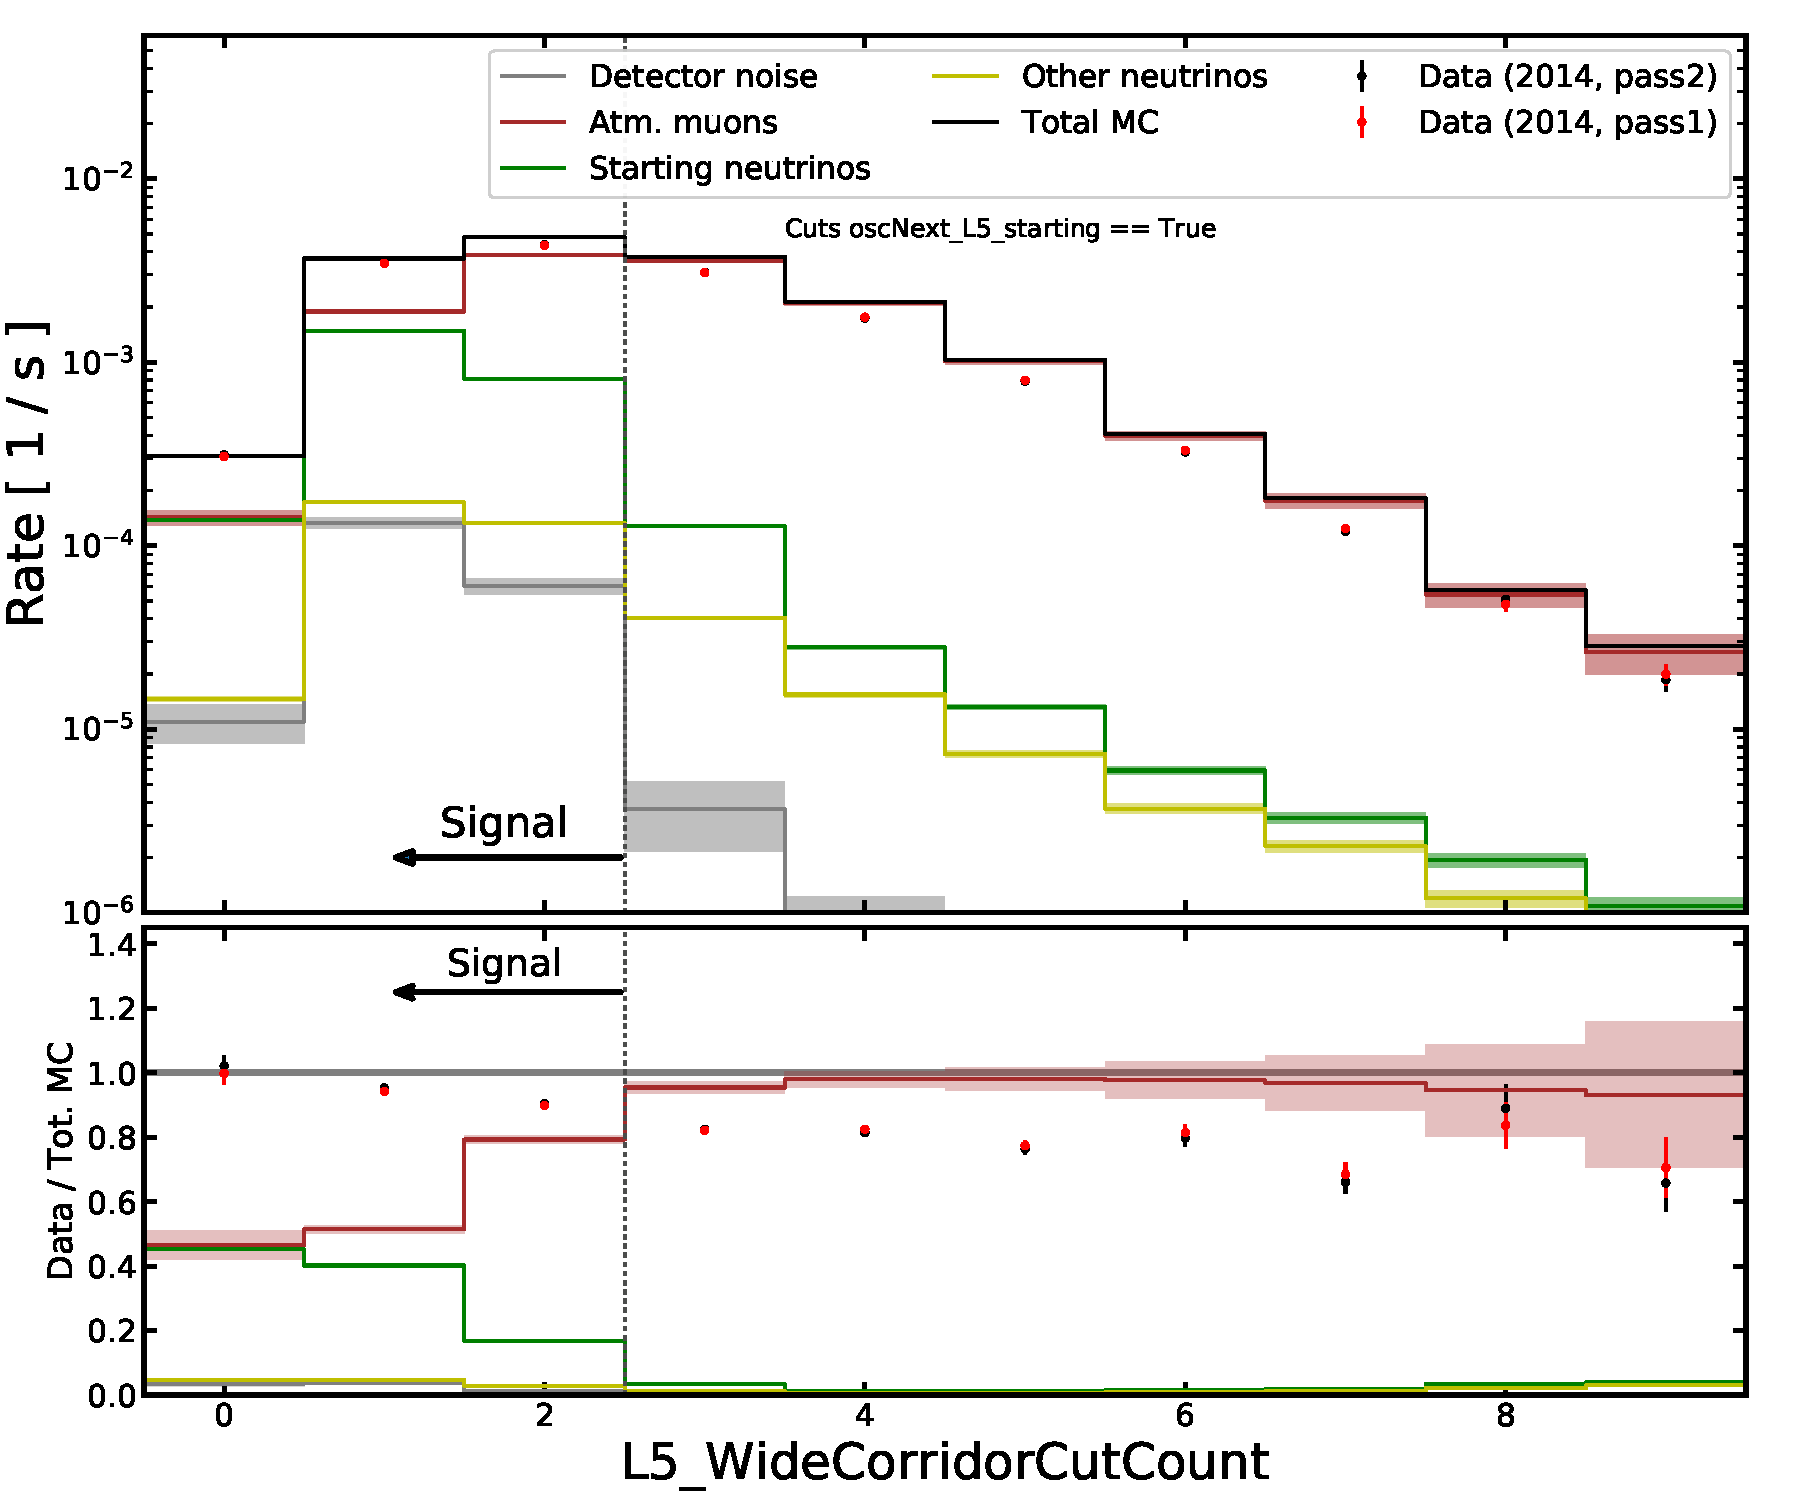
\includegraphics[width=7 cm]{figures/icecube/selection/L5_contained_L5_WideCorridorCutCount.pdf}
    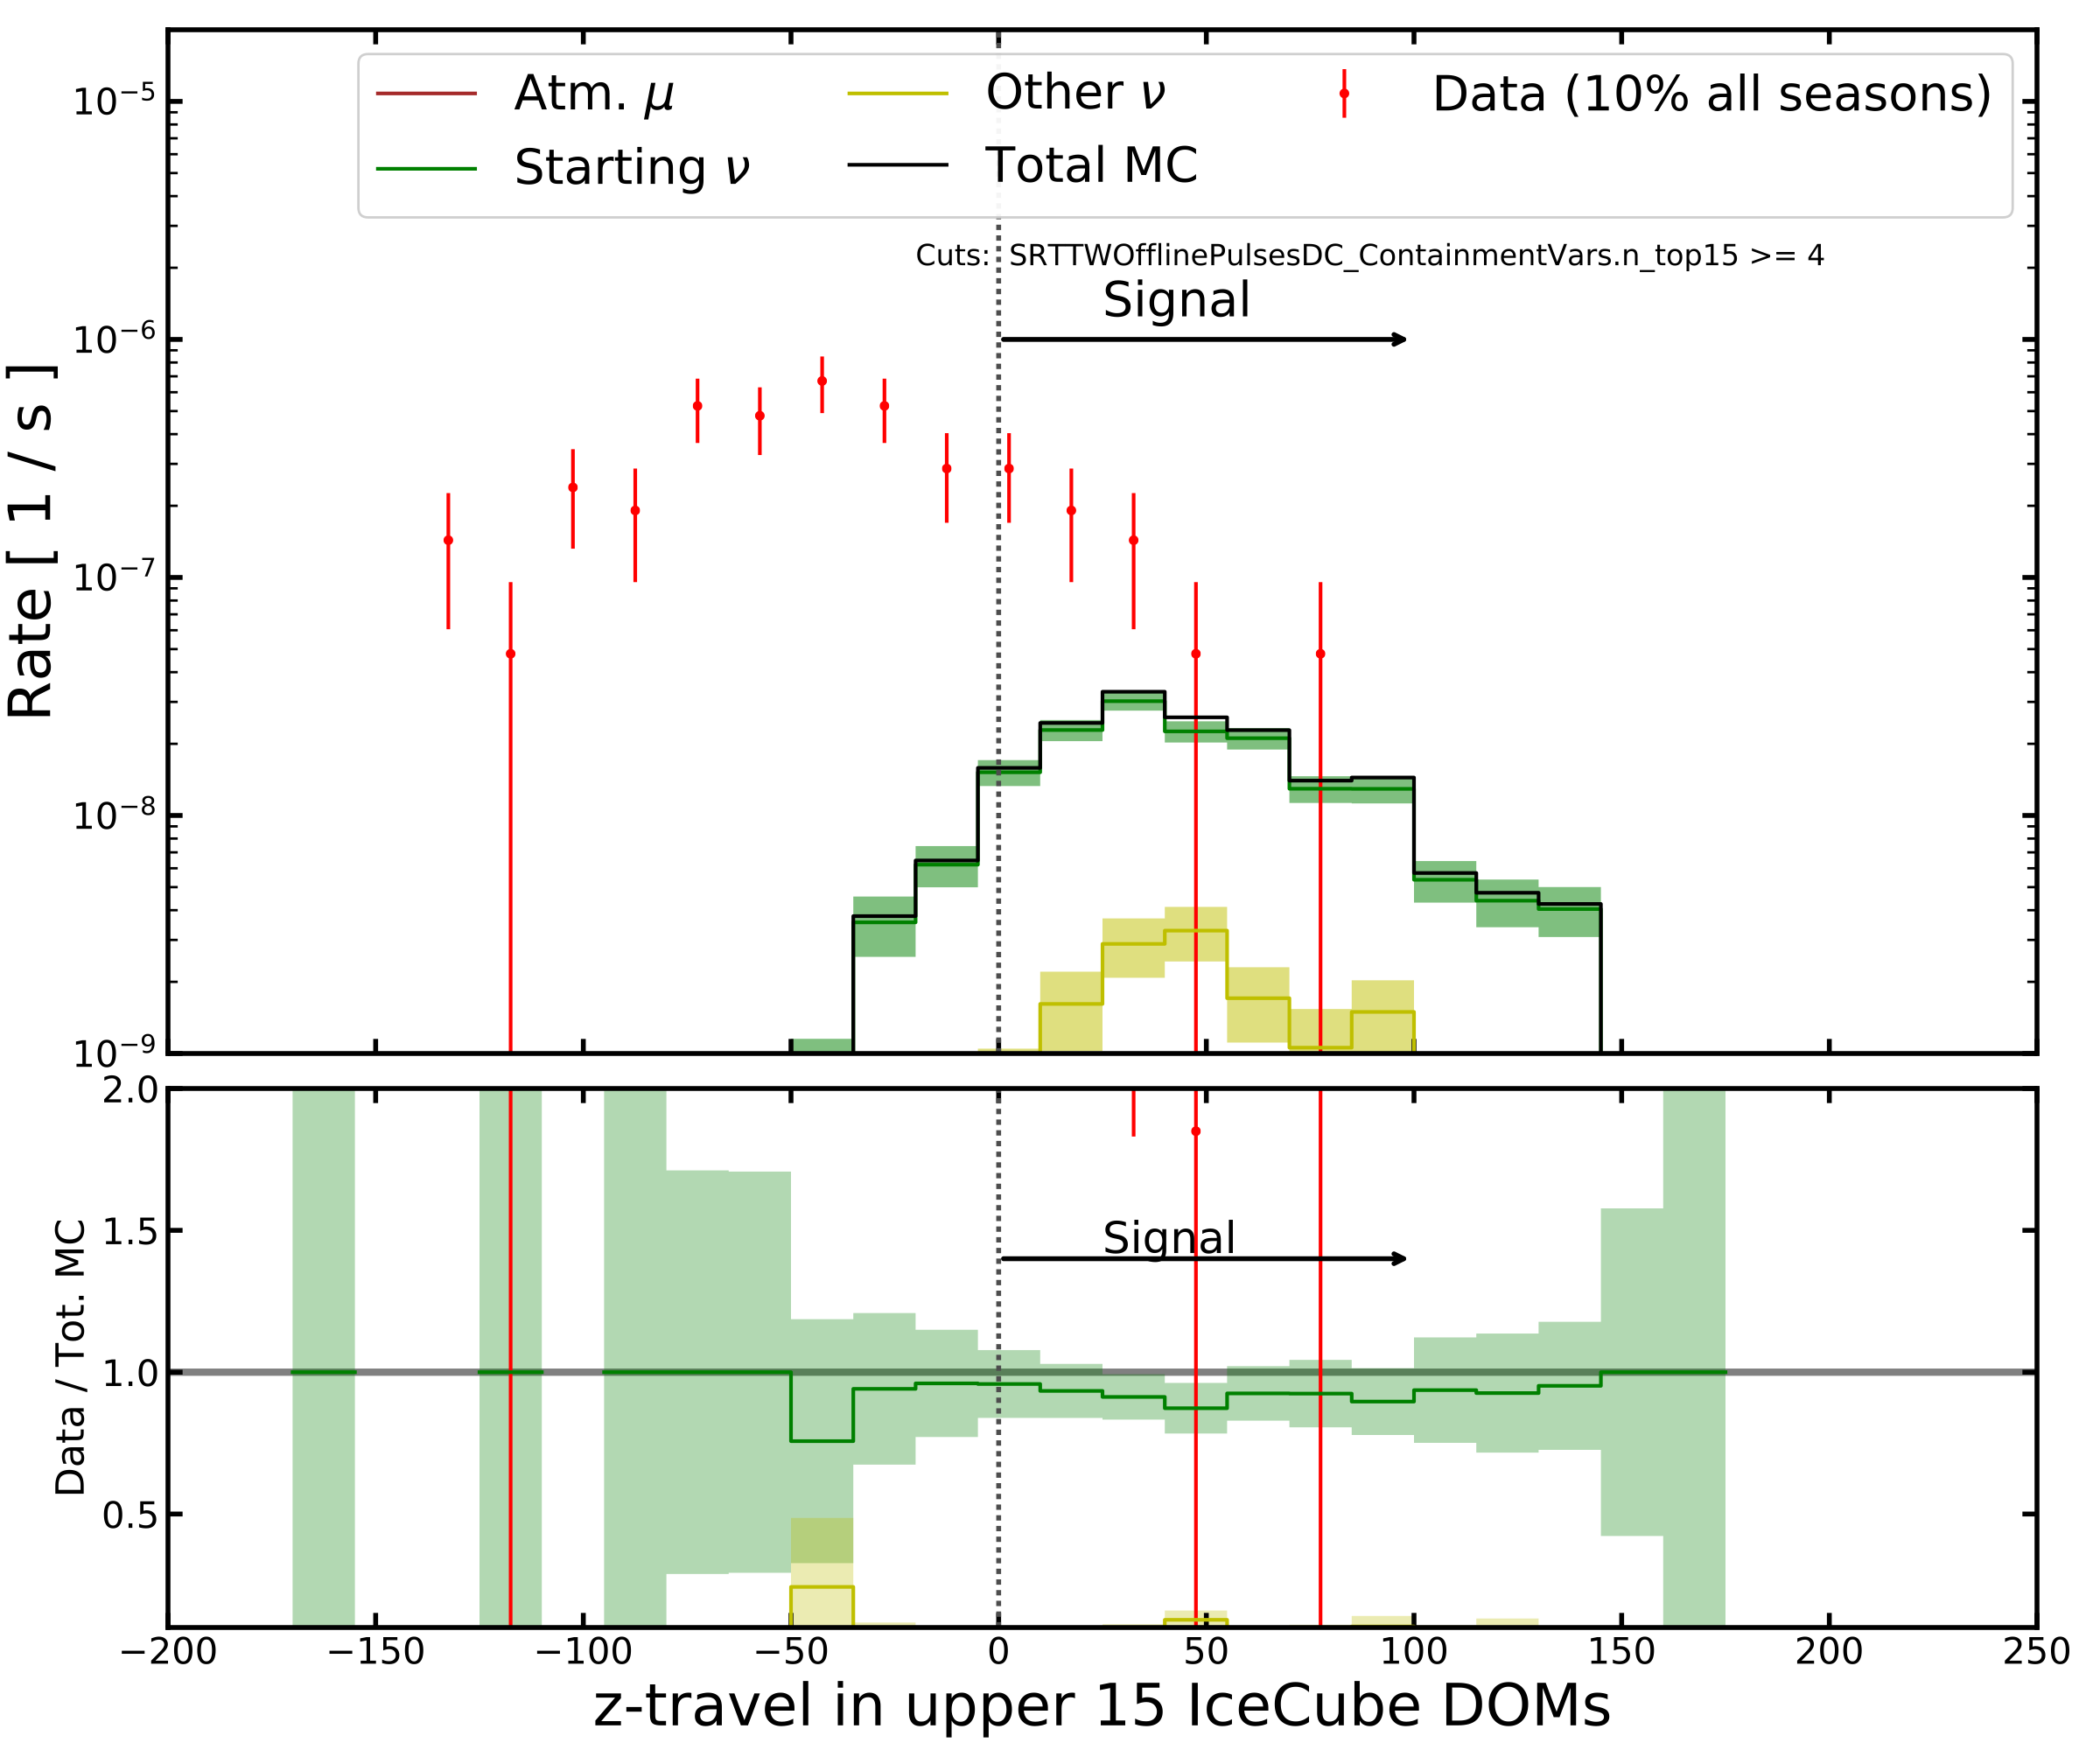
\includegraphics[width=7 cm]{figures/icecube/selection/SRTTWOfflinePulsesDC_ContainmentVars.z_travel_top15.png}
    \caption{Distributions for one of the L5 corridor cut variables (left) and one of the variables used to reject coincident muon events (right). The distribution in the right panel is shown only for events which have at least four hits in the uppermost 15 DOMs combined over all IceCube strings.}
    \label{fig:l5-vars}
\end{figure*}

\begin{table}
\begin{tabular}{lrrrrr}
Event type  & DC filter   & L3   & L4   & L5   & Eff. (\%) \\
\toprule
Atm. $\mu$         & 7273 & 505  & 28.1 & 0.93 & 0.012          \\
Pure noise         & 6621 & 36.6 & 0.28 & 0.07 & 0.001          \\
Atm. $\nu_e$ CC    & 1.61 & 0.95 & 0.84 & 0.48 & 29.8           \\
Atm. $\nu_\mu$ CC  & 6.16 & 3.77 & 3.11 & 1.39 & 22.5           \\
Atm. $\nu_\tau$ CC & 0.19 & 0.13 & 0.12 & 0.07 & 36.8           \\
Atm. $\nu$ NC      & 0.86 & 0.53 & 0.46 & 0.23 & 26.7  \\
\end{tabular}
\caption{Summary of the rates (in mHz) obtained after each level of selection. Neutrinos are weighted to an atmospheric spectrum with oscillations included.}
\label{tab:l5_summary}
\end{table}

\subsection{Event Reconstruction}
\label{sec:event-reconstruction}

After the L5 selection, the rate of muons is reduced enough such that the majority of the total sample is expected to consist of atmospheric neutrinos, and it is at this point that the event reconstruction and signature classification is run. For the measurement presented in this thesis, three reconstructed quantities are required: The zenith angle, the energy, and a proxy score that determines the flavor of a neutrino. As described in section \ref{sec:particle-signatures}, all neutrino events in DeepCore can be effectively approximated as either a cascade ($\nu_e$ CC events, all NC events, and 83\% of $\nu_\tau$ CC events) or a combination of a cascade at the neutrino interaction point with an out-going muon track ($\nu_\mu$ CC events and 17\% of $\nu_\tau$ CC events). The zenith angle can be most accurately reconstructed for track-like events due to their elongated, highly directional signature. For cascades, the reconstruction of the direction is more difficult because of their most compact and diffuse light distribution. The energy of a neutrino event is reconstructed by comparing the expected light output of a combined track and cascade hypothesis to the observed hits. Finally, the flavor proxy is calculated using variables that characterize the elongation of the observed hit signature  and the goodness-of-fit of a combined track and cascade hypothesis compared to that of a cascade-only hypothesis. The resulting score allows the separation of muon neutrino interactions from other interactions, which is ideally suitable to observe the muon neutrino disappearance oscillation channel.

\subsubsection{Zenith angle reconstruction}
The zenith is reconstructed using an old but refurbished algorithm that first removes hits from light that is likely to have undergone a significant amount of scattering and then runs a modified $\chi^2$ fit on the observation times of the remaining hits assuming that they all lie on a Cherenkov cone that would be produced by a minimally ionizing muon. Because of the required hit cleaning step, not all events present at L5 can be reconstructed in this way. However, those events that pass the cleaning condition are the cleanest, most track-like events of the entire sample and therefore can be seen as a high-quality "golden sample".


